\subsection{Optimizadores de Lote Grande, Eficientes en Memoria y Sin Tasa de Aprendizaje}
\paragraph{LAMB (Layer-wise Adaptive Moments optimizer for Batch training).}
\begin{figure}[H]
\centering
\fitfigure{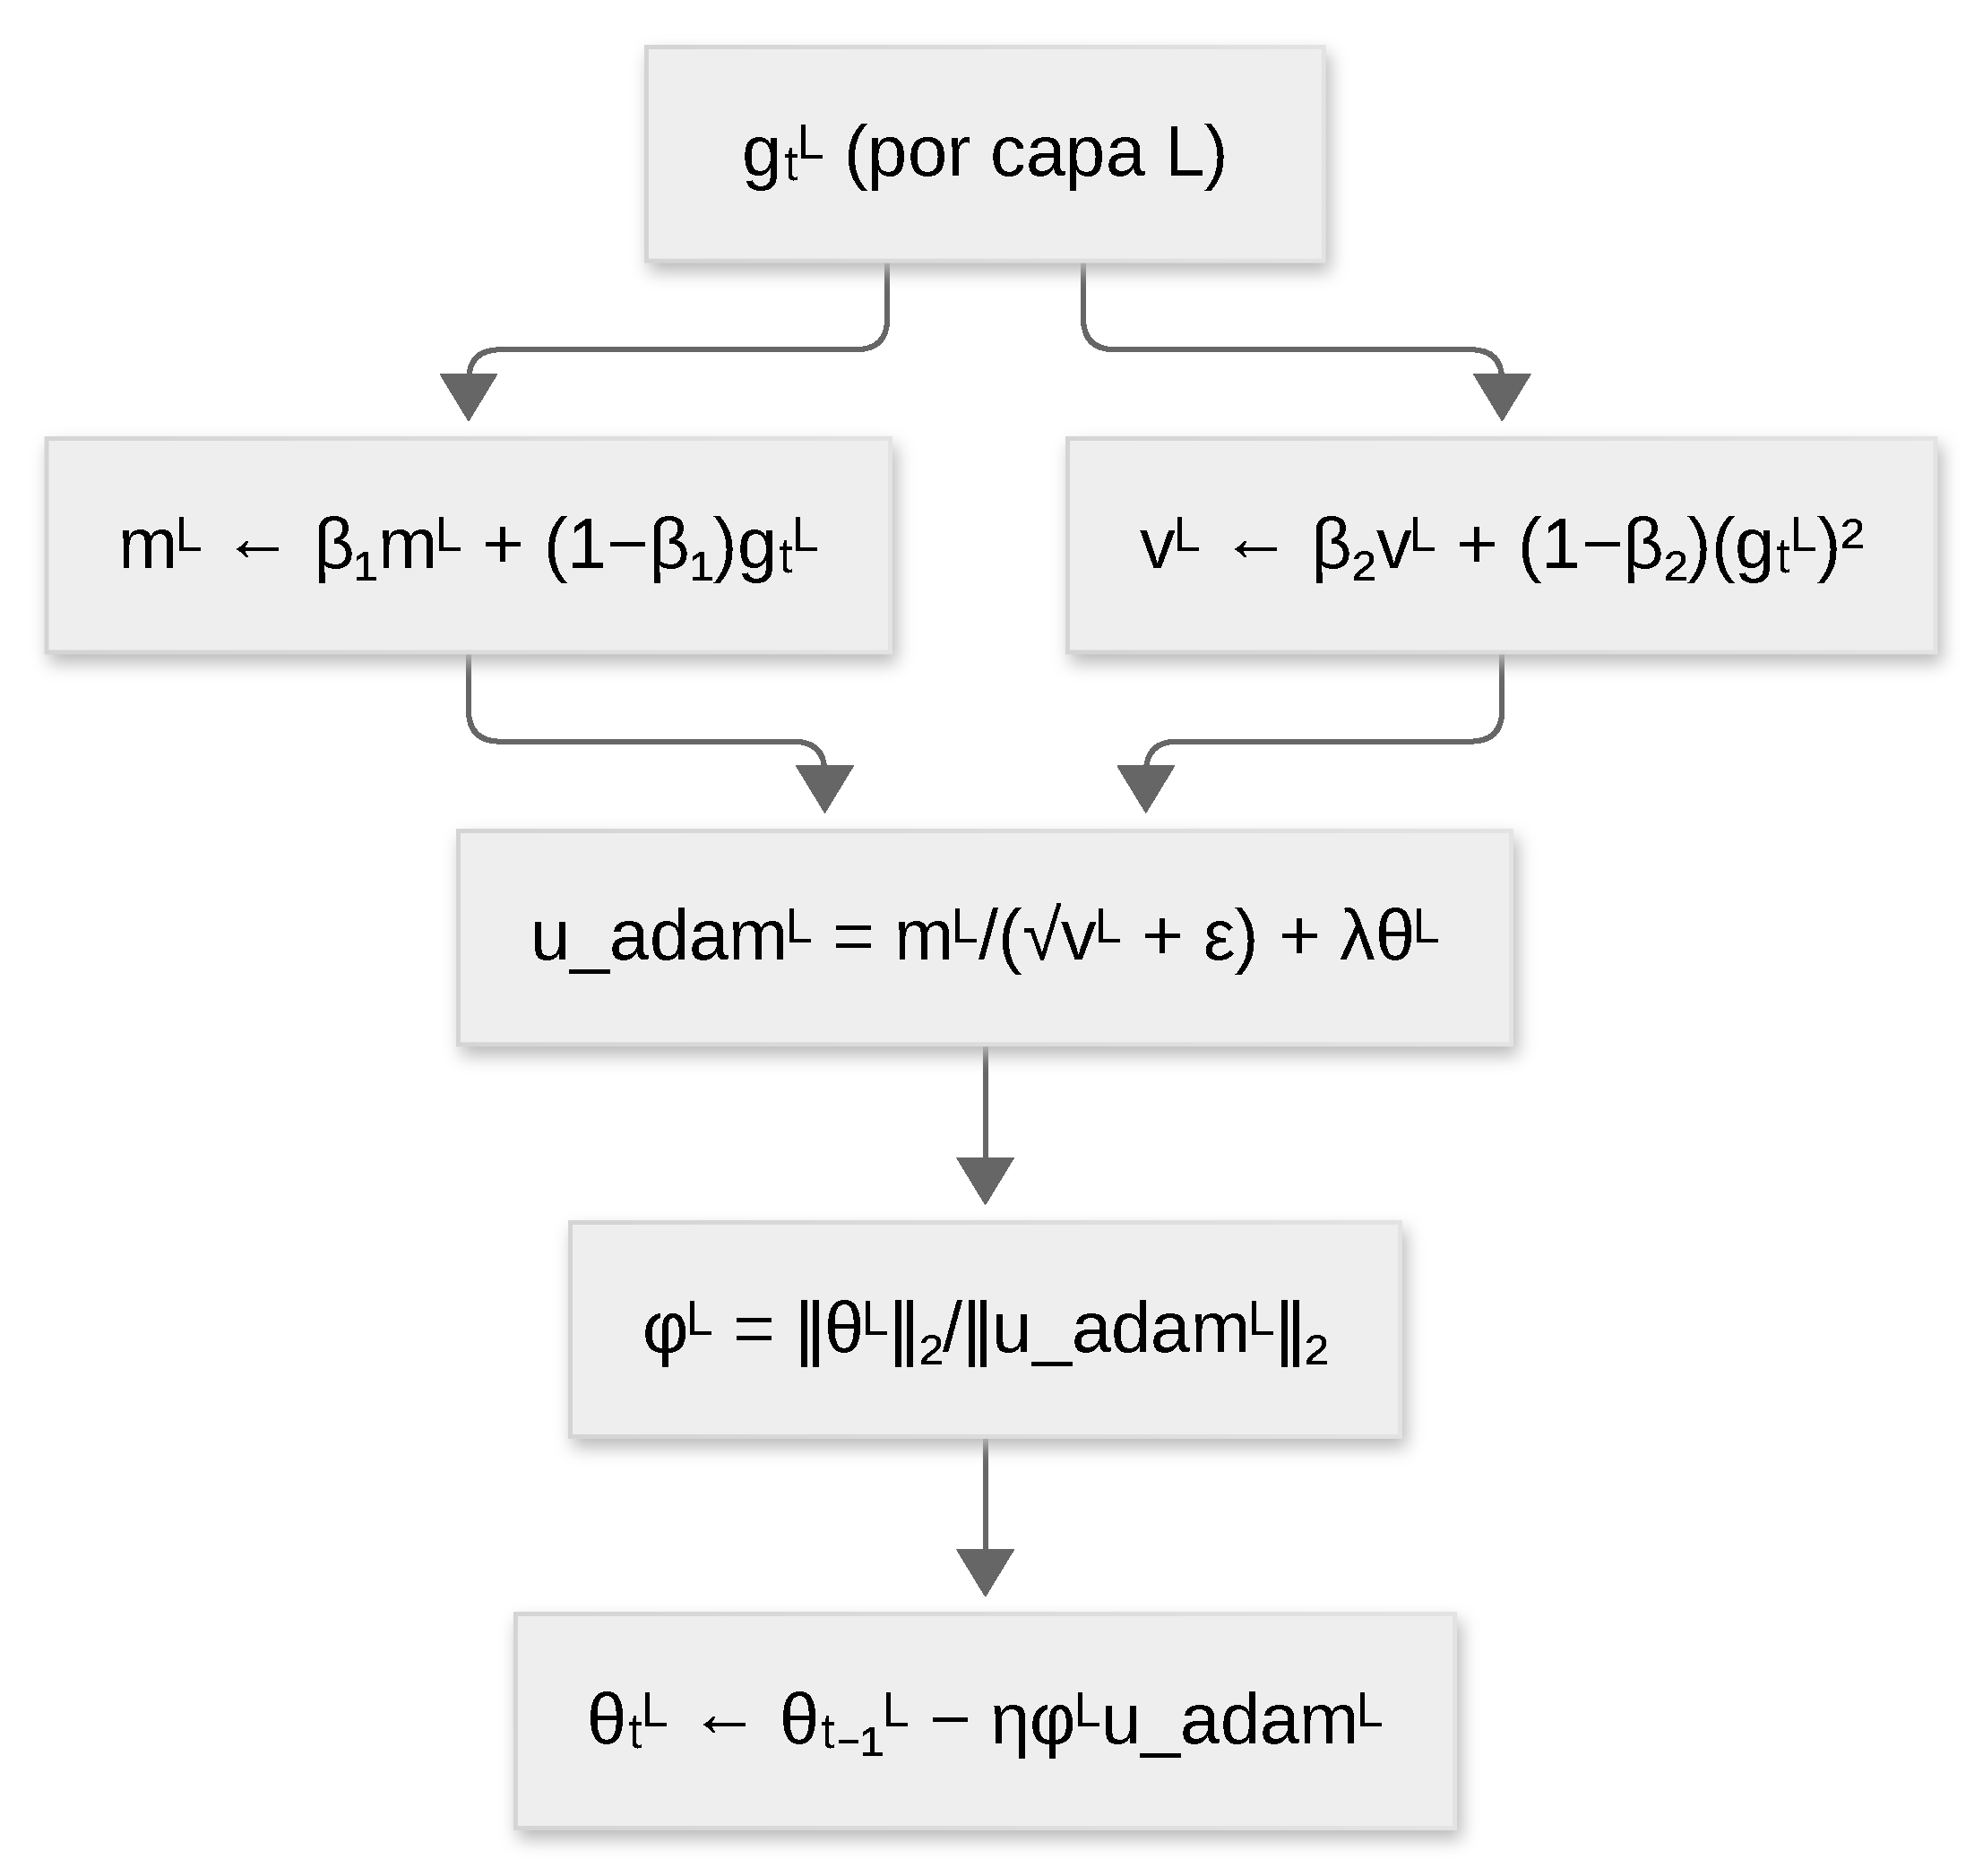
\includegraphics{../paper/figures/optimizers/lamb-es.pdf}}
\caption{Flujo por paso de LAMB: paso Adam por capas reescalado por la razón de confianza entre las normas de pesos y actualización.}
\label{fig:opt-lamb}
\end{figure}
LAMB extiende Adam con \textbf{escalado de tasa adaptativo por capas} (inspirado en LARS), permitiendo entrenamiento estable con tamaños de lote extremos (e.g., 64K en BERT):
\begin{align}
m_t^L &= \beta_1 m_{t-1}^L + (1-\beta_1)g_t^L \quad\text{(momento de primer orden por capas)} \\
v_t^L &= \beta_2 v_{t-1}^L + (1-\beta_2)(g_t^L)^2 \\
u_{\text{adam}}^L &= \frac{m_t^L}{\sqrt{v_t^L}+\epsilon} + \lambda\theta_{t-1}^L \quad\text{(paso adaptativo base con decaimiento)} \\
\phi^L &= \frac{\|\theta_{t-1}^L\|_2}{\|u_{\text{adam}}^L\|_2} \quad\text{(razón de confianza: normalización por capas)} \\
\theta_t^L &= \theta_{t-1}^L - \eta \cdot \phi^L \cdot u_{\text{adam}}^L
\end{align}
La \textbf{razón de confianza} $\phi^L = \|\theta^L\|_2 / \|u_{\text{adam}}^L\|_2$ normaliza el paso de actualización efectivo en relación con la magnitud de los pesos. En lotes muy grandes, el ruido estocástico del gradiente puede superar a la señal, desestabilizando las tasas de aprendizaje por capas. Al escalar las actualizaciones proporcionalmente a las normas de los pesos, LAMB asegura cambios relativos en lugar de absolutos, evitando que actualizaciones pequeñas y seguras en vectores grandes dominen.

\begin{algorithm}[H]
\caption{LAMB (Layer-wise Adaptive Moments optimizer for Batch training)}
\label{alg:lamb}
\begin{algorithmic}[1]
\Require Parámetros iniciales $\theta_0$, tasa de aprendizaje $\eta$, $\beta_1, \beta_2$, decaimiento de pesos $\lambda$
\Ensure Parámetros actualizados $\theta_T$
\State Inicializar: Para cada capa $L$: $m^L \gets 0$, $v^L \gets 0$
\For{$t = 1, 2, \ldots, T$}
    \For{cada capa $L$}
        \State $g_t^L \gets \nabla f(\theta_t^L)$
        \State $m^L \gets \beta_1 m^L + (1-\beta_1) g_t^L$
        \State $v^L \gets \beta_2 v^L + (1-\beta_2) (g_t^L)^2$
        \State Adam base: $u_{\text{adam}}^L \gets m^L / (\sqrt{v^L} + \epsilon)$
        \If{weight\_decay $> 0$}
            \State $u_{\text{adam}}^L \gets u_{\text{adam}}^L + \lambda \theta_{t-1}^L$
        \EndIf
        \State Razón de confianza: $\phi^L \gets \|\theta_{t-1}^L\|_2 / \|u_{\text{adam}}^L\|_2$ si ambos son no nulos, sino $1$
        \State $\theta_t^L \gets \theta_{t-1}^L - \eta \phi^L u_{\text{adam}}^L$
    \EndFor
\EndFor
\Return $\theta_T$
\end{algorithmic}
\end{algorithm}

\paragraph{Contras.}
\begin{itemize}[leftmargin=*]
\item La contabilidad de normas por capas y el cálculo de la razón de confianza añaden sobrecarga por paso.
\item La razón de confianza es inestable cuando las normas de capa o de actualización son cercanas a cero.
\end{itemize}

\paragraph{Ventajas.}
\begin{itemize}[leftmargin=*]
\item Permite entrenamiento estable con tamaños de lote extremos (e.g., 64K en BERT).
\item Preserva los beneficios de generalización de lotes pequeños mientras escala el lote.
\end{itemize}

\paragraph{Schedule-Free AdamW.}
\begin{figure}[H]
\centering
\fitfigure{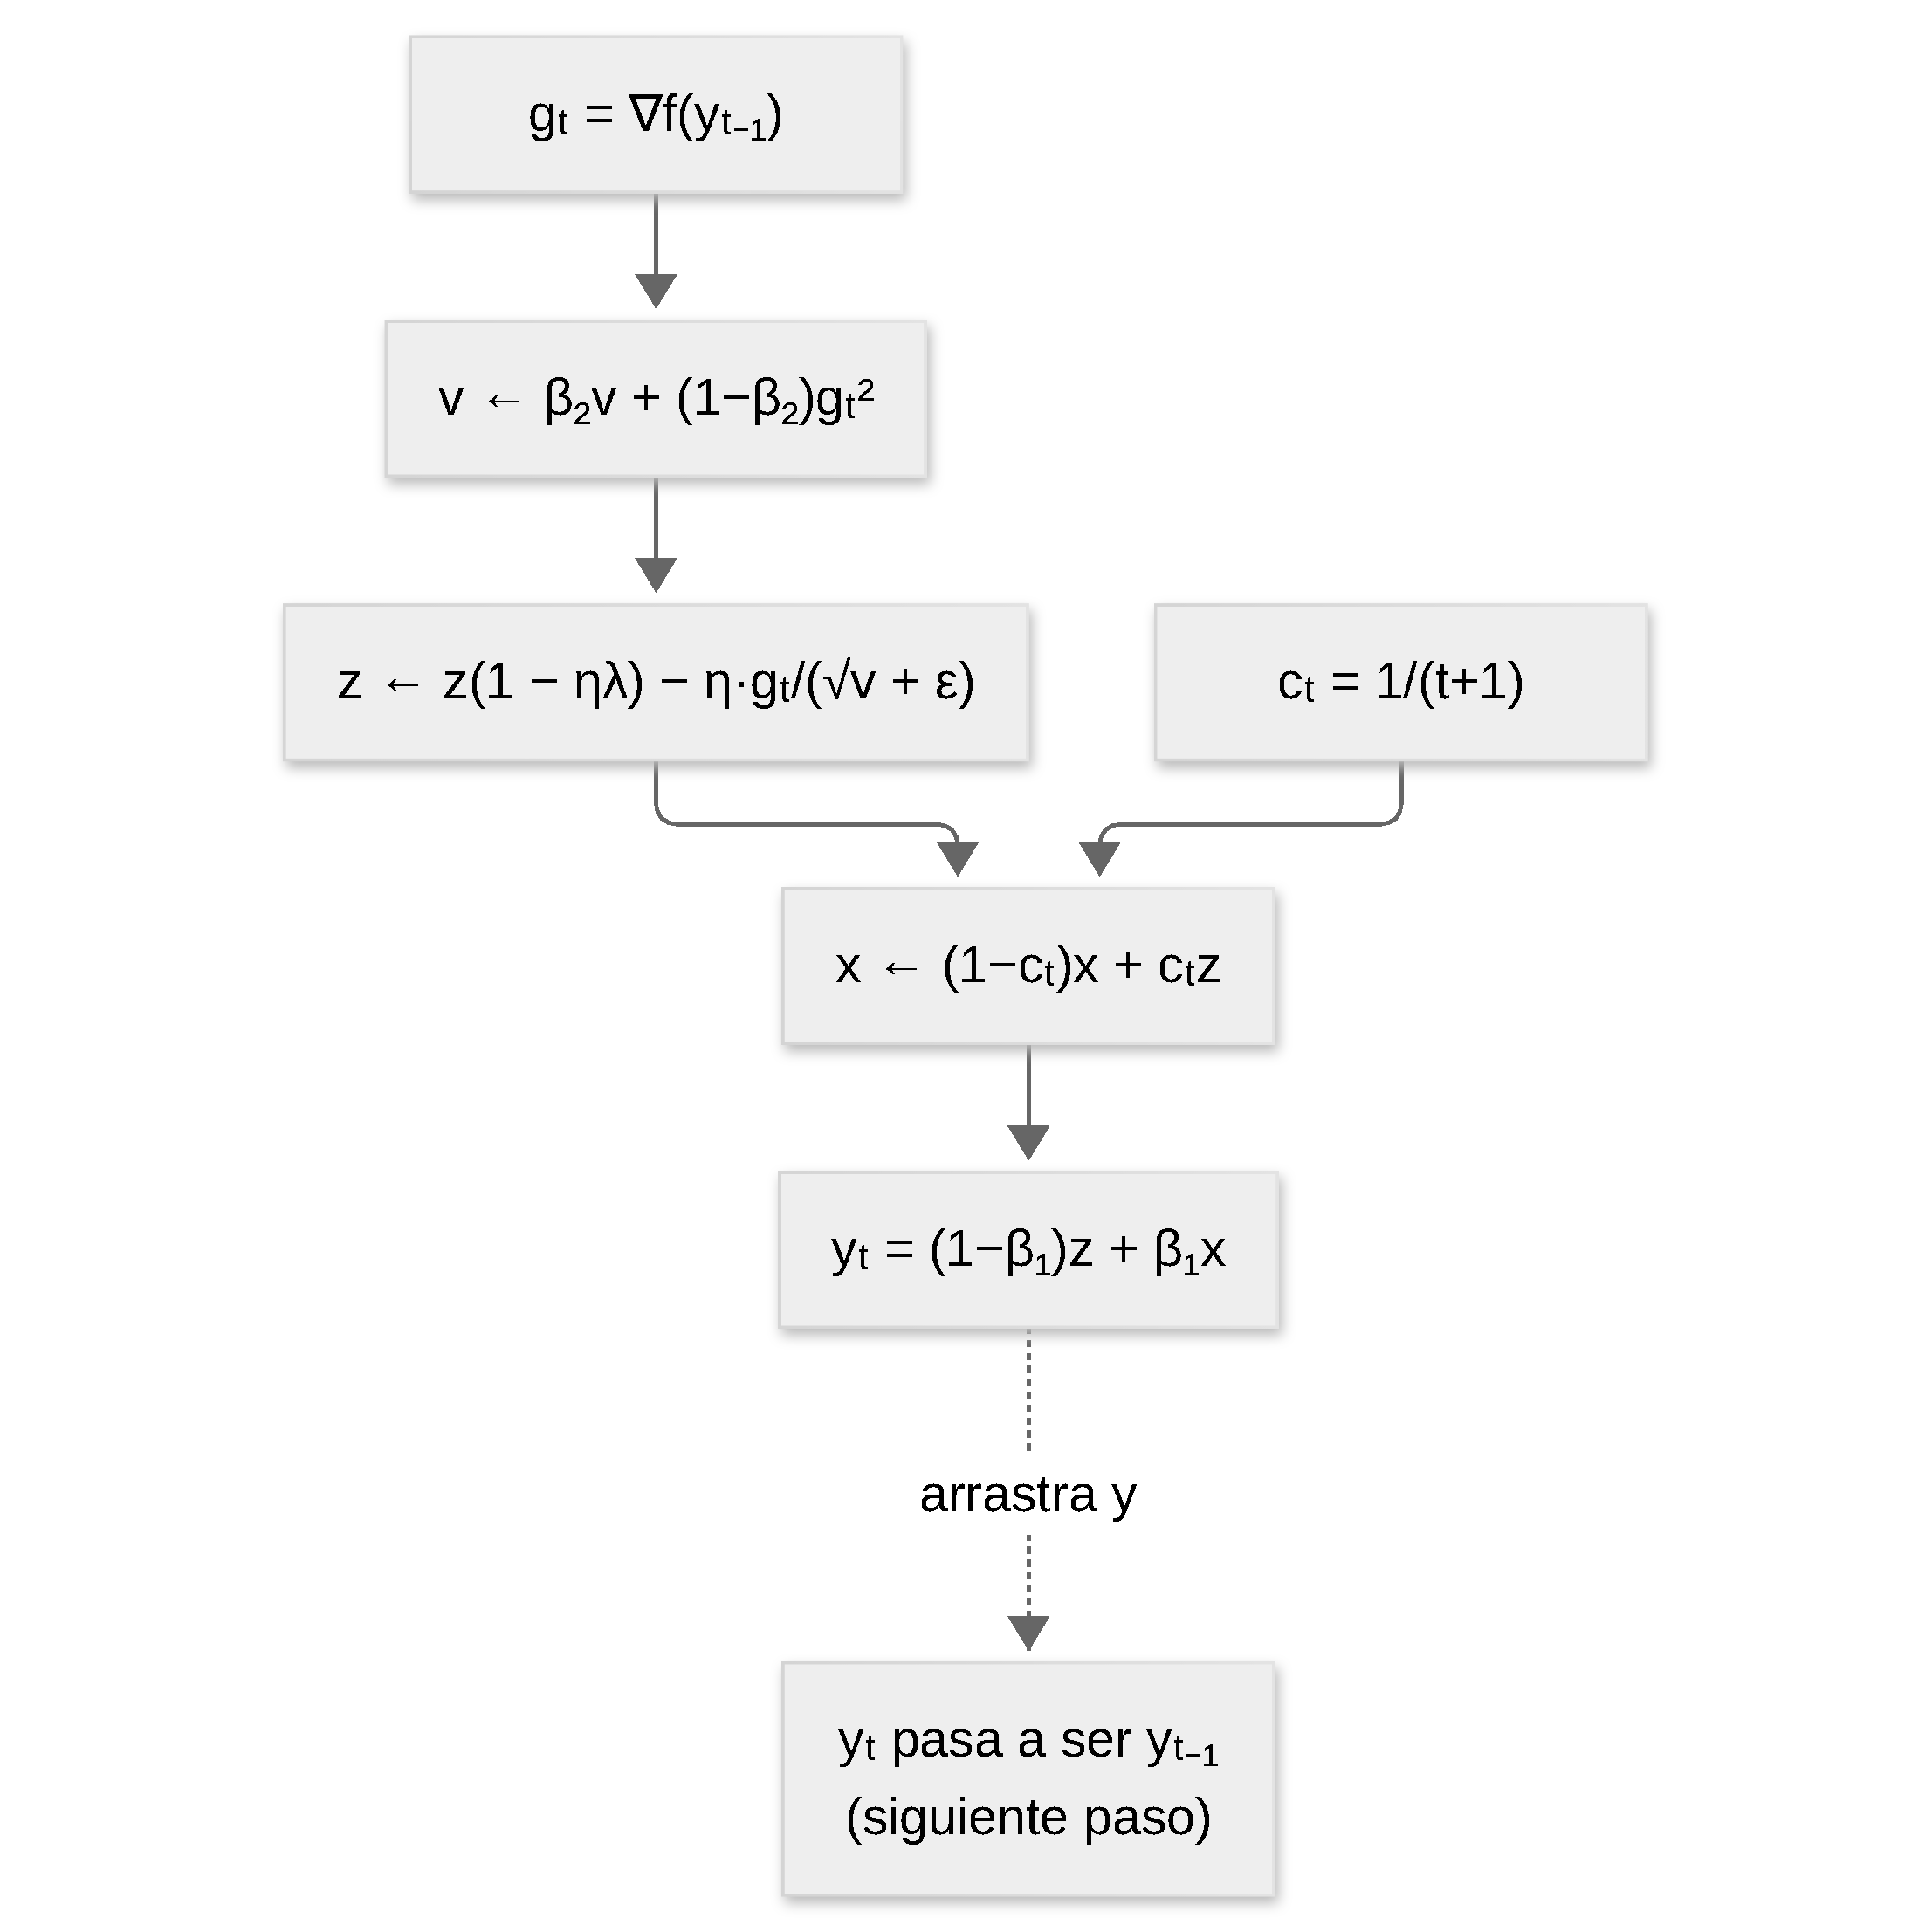
\includegraphics{../paper/figures/optimizers/schedulefree-es.pdf}}
\caption{Flujo por paso de Schedule-Free AdamW: flujo de exploración $z$, promedio de iteraciones $x$ y punto de interpolación $y$, con promediado implícito $1/(t+1)$.}
\label{fig:opt-schedulefree}
\end{figure}
Los métodos Schedule-Free eliminan el diseño explícito de programación de la receta de optimización. El algoritmo mantiene dos flujos de parámetros: $z_t$ (exploración) y $x_t$ (promedio suavizado):
\begin{align}
v_t &= \beta_2 v_{t-1} + (1-\beta_2)g_t^2 \quad\text{(varianza)} \\
z_t &= z_{t-1}(1-\eta\lambda) - \eta\frac{g_t}{\sqrt{v_t}+\epsilon} \quad\text{(paso adaptativo con decaimiento)} \\
c_t &= \frac{1}{t+1} \quad\text{(coeficiente de promediado, decrece con el tiempo)} \\
x_t &= (1-c_t)x_{t-1} + c_t z_t \quad\text{(promediado de iteraciones)} \\
y_t &= (1-\beta)z_t + \beta x_t \quad\text{(interpolación para el punto de evaluación)}
\end{align}
El coeficiente de promediado $c_t = 1/(t+1)$ implementa una programación de tasa de aprendizaje implícita sin especificar explícitamente el número total de pasos $T$. Este marco unifica la programación y el promediado de iteraciones: el algoritmo explora mediante $z_t$ mientras acumula dirección estable mediante $x_t$. El punto de evaluación $y_t$ (usado para el cómputo del gradiente) interpola entre exploración y estabilidad.

\begin{algorithm}[H]
\caption{Schedule-Free AdamW}
\label{alg:schedulefree}
\begin{algorithmic}[1]
\Require Parámetros iniciales $\theta_0$, tasa de aprendizaje $\eta$ (fija), $\beta_1, \beta_2$, decaimiento de pesos $\lambda$
\Ensure Parámetros actualizados $\theta_T$ o promediado $x_T$
\State Inicializar: $z \gets \theta_0$ (exploración), $x \gets \theta_0$ (promedio), $v \gets 0$, $t \gets 0$
\For{$t = 1, 2, \ldots, T$}
    \State $g_t \gets \nabla f(y_{t-1})$ (gradiente en el punto de interpolación)
    \State $v \gets \beta_2 v + (1-\beta_2) g_t^2$ \Comment{Varianza}
    \State Decaimiento de pesos sobre $z$: $z \gets z(1 - \eta\lambda)$
    \State $z \gets z - \eta g_t / (\sqrt{v} + \epsilon)$ \Comment{Paso adaptativo sobre el gradiente crudo}
    \State $c_t \gets 1 / (t+1)$ \Comment{Coeficiente de promediado}
    \State $x \gets (1-c_t) x + c_t z$ \Comment{Promediado de iteraciones}
    \State $y_t \gets (1-\beta_1) z + \beta_1 x$ \Comment{Interpolación para la siguiente evaluación}
\EndFor
\Return $x_T$ o $y_T$
\end{algorithmic}
\end{algorithm}

\paragraph{Contras.}
\begin{itemize}[leftmargin=*]
\item Mantiene dos flujos de parámetros ($z$ y $x$) y requiere manejar explícitamente el punto de evaluación.
\item Su comportamiento difiere de las líneas base con programación, lo que complica las comparaciones.
\end{itemize}

\paragraph{Ventajas.}
\begin{itemize}[leftmargin=*]
\item Elimina la programación explícita de la tasa de aprendizaje y su hiperparámetro de pasos totales.
\item Convergencia de última generación en optimización convexa, aprendizaje profundo a gran escala y aprendizaje por refuerzo.
\end{itemize}

\paragraph{Adafactor.}
\begin{figure}[H]
\centering
\fitfigure{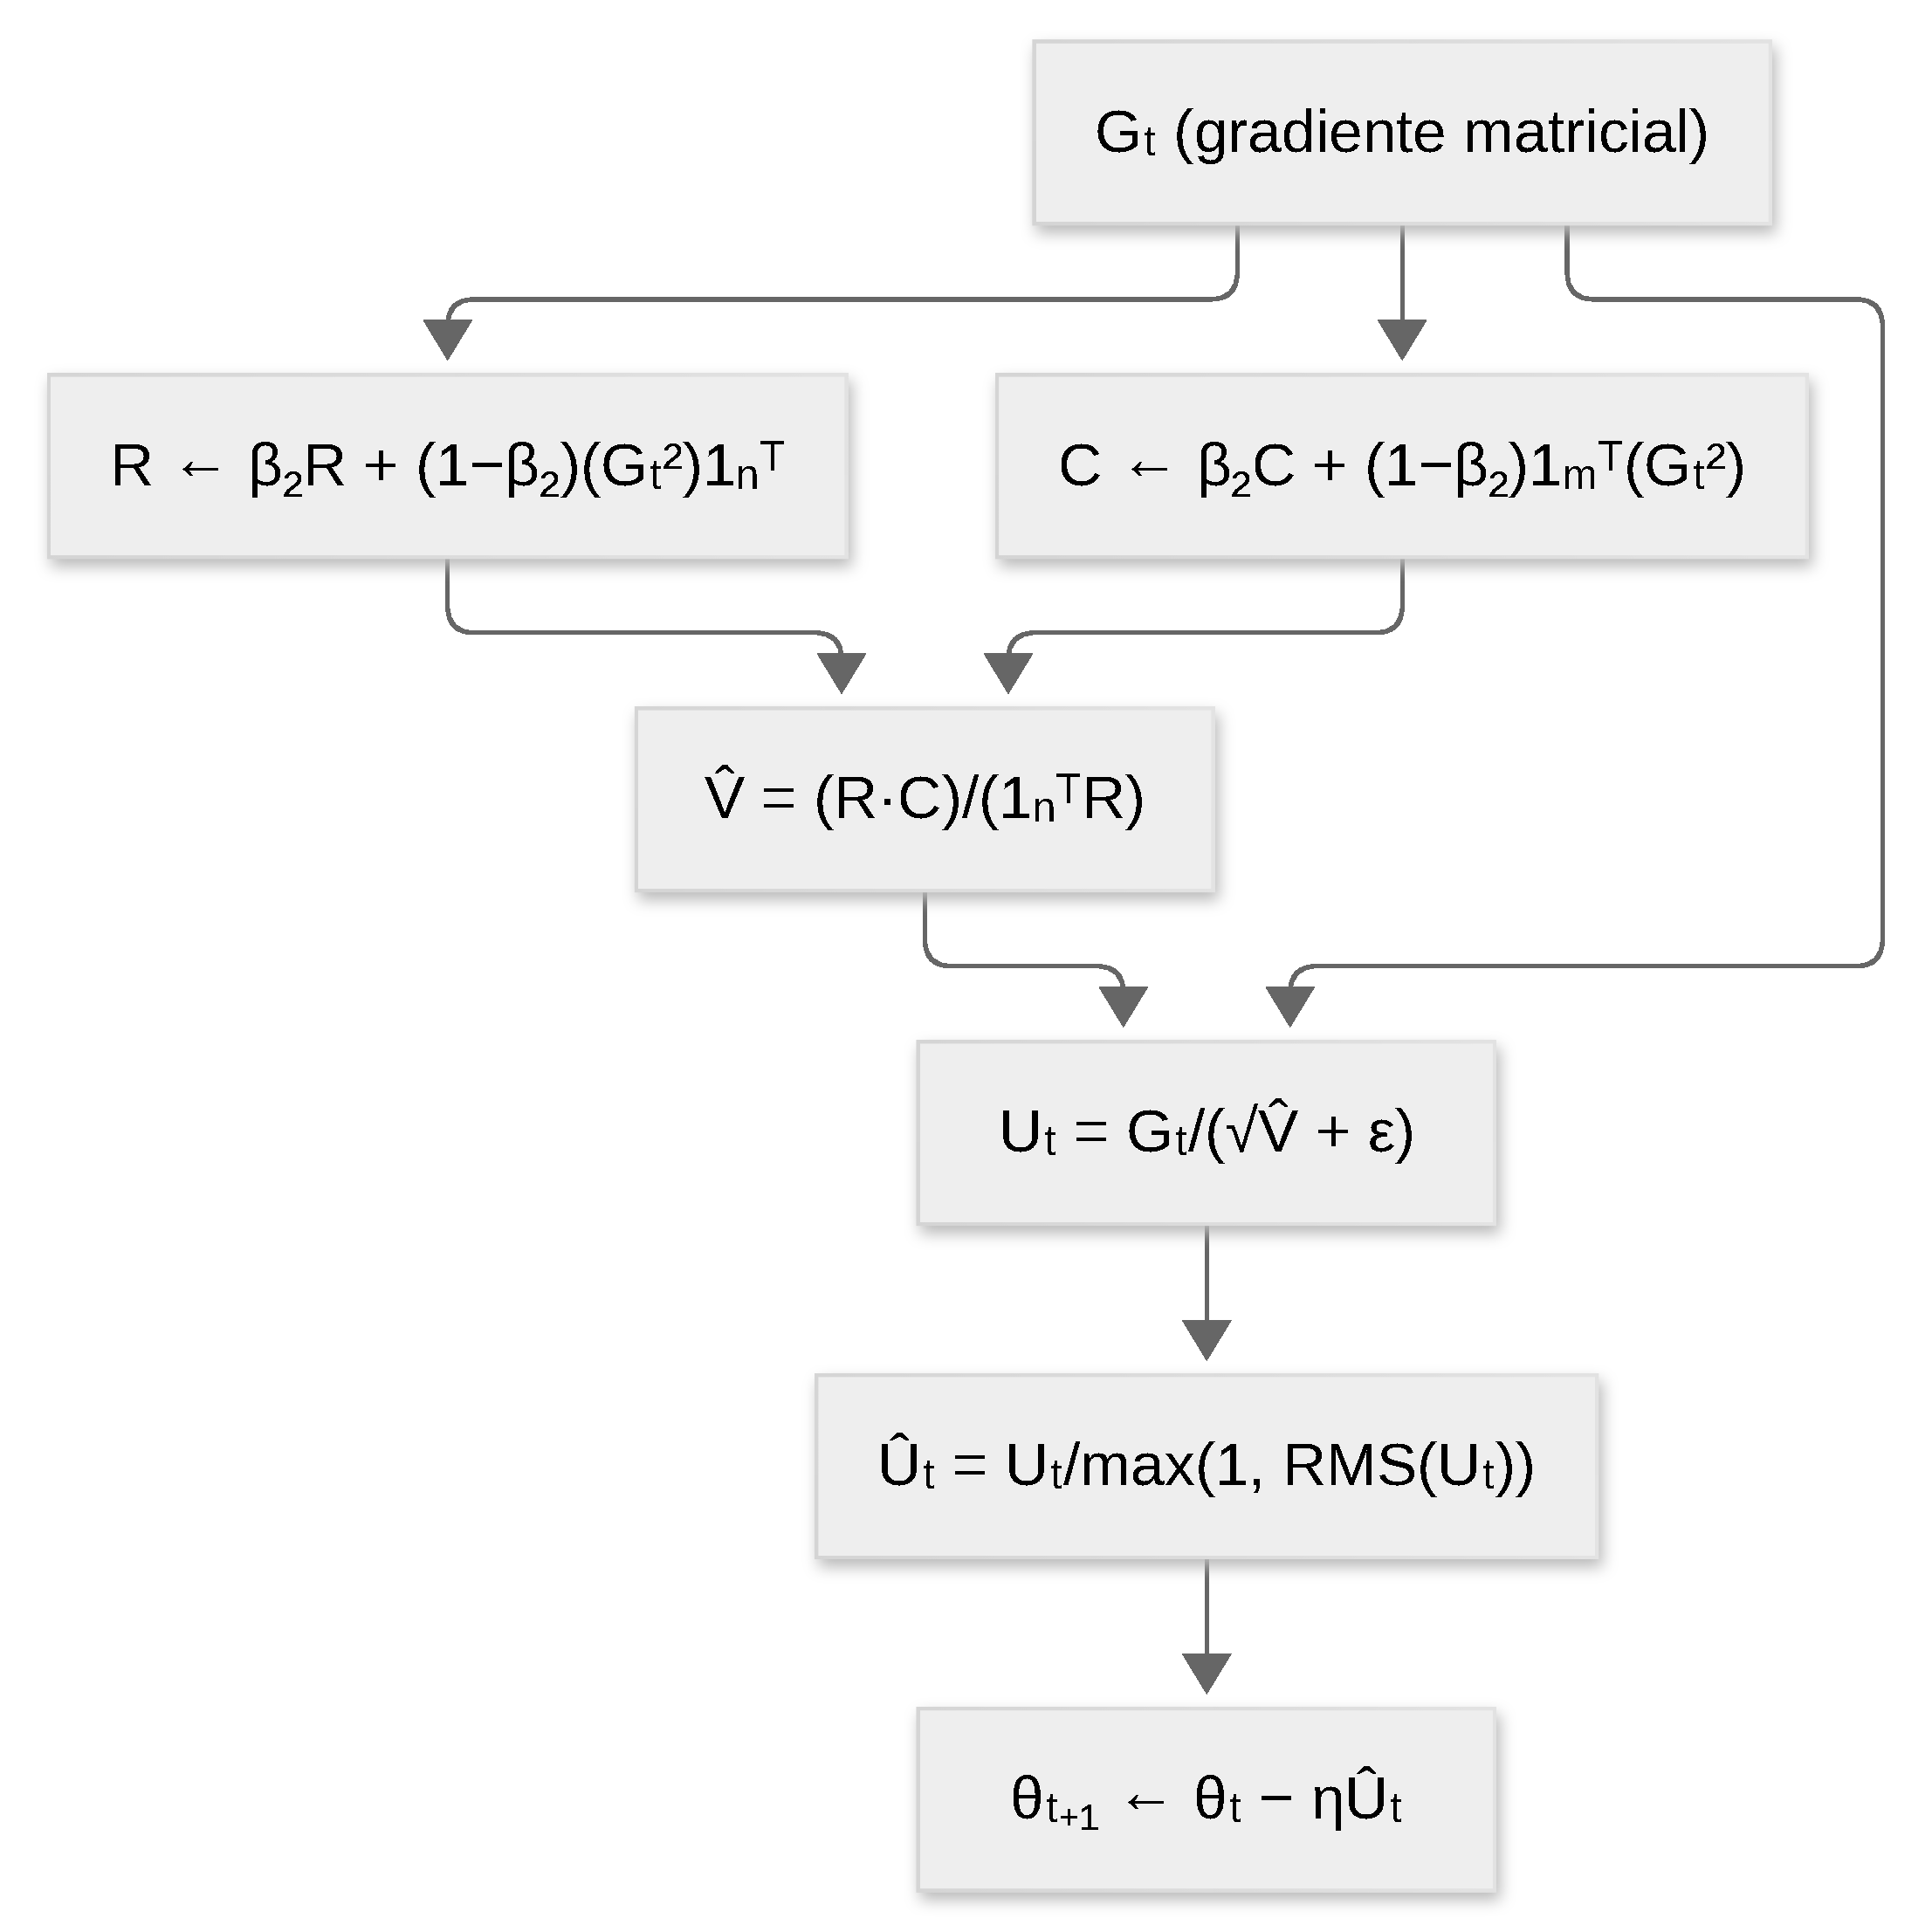
\includegraphics{../paper/figures/optimizers/adafactor-es.pdf}}
\caption{Flujo por paso de Adafactor: acumuladores factorizados de segundo momento por filas y columnas, reconstrucción mediante producto exterior y recorte RMS.}
\label{fig:opt-adafactor}
\end{figure}
Adafactor reduce la memoria del optimizador \textbf{factorizando} estadísticas de segundo momento para parámetros con forma de matriz, almacenando solo acumuladores de filas y columnas en lugar de estados de varianza densos. Para una matriz de gradiente $G_t \in \mathbb{R}^{m \times n}$:
\begin{align}
R_t &= \beta_2 R_{t-1} + (1-\beta_2)(G_t^2) \mathbf{1}_n^T \quad\text{(varianza por filas)} \\
C_t &= \beta_2 C_{t-1} + (1-\beta_2) \mathbf{1}_m^\top (G_t^2) \quad\text{(varianza por columnas)} \\
\hat{V}_t &= \frac{R_t C_t}{\mathbf{1}_n^\top R_t} \quad\text{(varianza reconstruida mediante producto exterior)} \\
U_t &= \frac{G_t}{\sqrt{\hat{V}_t}+\epsilon} \quad\text{(paso adaptativo normalizado)} \\
\hat{U}_t &= \frac{U_t}{\max(1, \text{RMS}(U_t))} \quad\text{(recorte de estabilidad)}
\end{align}

\begin{algorithm}[H]
\caption{Adafactor (Estadísticas de Segundo Momento Factorizadas)}
\label{alg:adafactor}
\begin{algorithmic}[1]
\Require Matriz de gradiente $G_t \in \mathbb{R}^{m \times n}$, tasa de aprendizaje $\eta$, $\beta_2 \approx 0.999$
\Ensure Parámetros actualizados $\theta_T$
\State Inicializar: Acumuladores de fila $R \gets \epsilon \mathbf{1}^T_m$, Columna $C \gets \epsilon \mathbf{1}_n$
\For{$t = 1, 2, \ldots, T$}
    \State $G_t \gets \nabla f(\theta_t)$ (gradiente matricial)
    \State $R \gets \beta_2 R + (1-\beta_2) (G_t^2) \mathbf{1}_n^T$ \Comment{Productos internos por filas}
    \State $C \gets \beta_2 C + (1-\beta_2) \mathbf{1}_m^\top (G_t^2)$ \Comment{Productos internos por columnas}
    \State Varianza reconstruida: $\hat{V} \gets (R \cdot C) / (\mathbf{1}_n^\top R)$ \Comment{Mediante producto exterior}
    \State Paso adaptativo normalizado: $U_t \gets G_t / (\sqrt{\hat{V}} + \epsilon)$
    \State Recorte RMS por fila: $\hat{U}_t \gets U_t / \max(1, \text{RMS}(U_t))$
    \State $\theta_{t+1} \gets \theta_t - \eta \hat{U}_t$
\EndFor
\Return $\theta_T$
\end{algorithmic}
\end{algorithm}

\paragraph{Contras.}
\begin{itemize}[leftmargin=*]
\item La varianza factorizada es una aproximación y puede ser inestable en algunas tareas.
\item Menor expresividad de optimización en comparación con Adam completo.
\end{itemize}

\paragraph{Ventajas.}
\begin{itemize}[leftmargin=*]
\item La memoria baja de $O(n_{\text{params}})$ a $O(\sqrt{n_{\text{params}}})$ para parámetros matriciales.
\item Más atractivo cuando la VRAM está dominada por el estado del optimizador en lugar de las activaciones.
\end{itemize}

\paragraph{GaLore (Gradient Low-Rank Projection).}
\begin{figure}[H]
\centering
\fitfigure{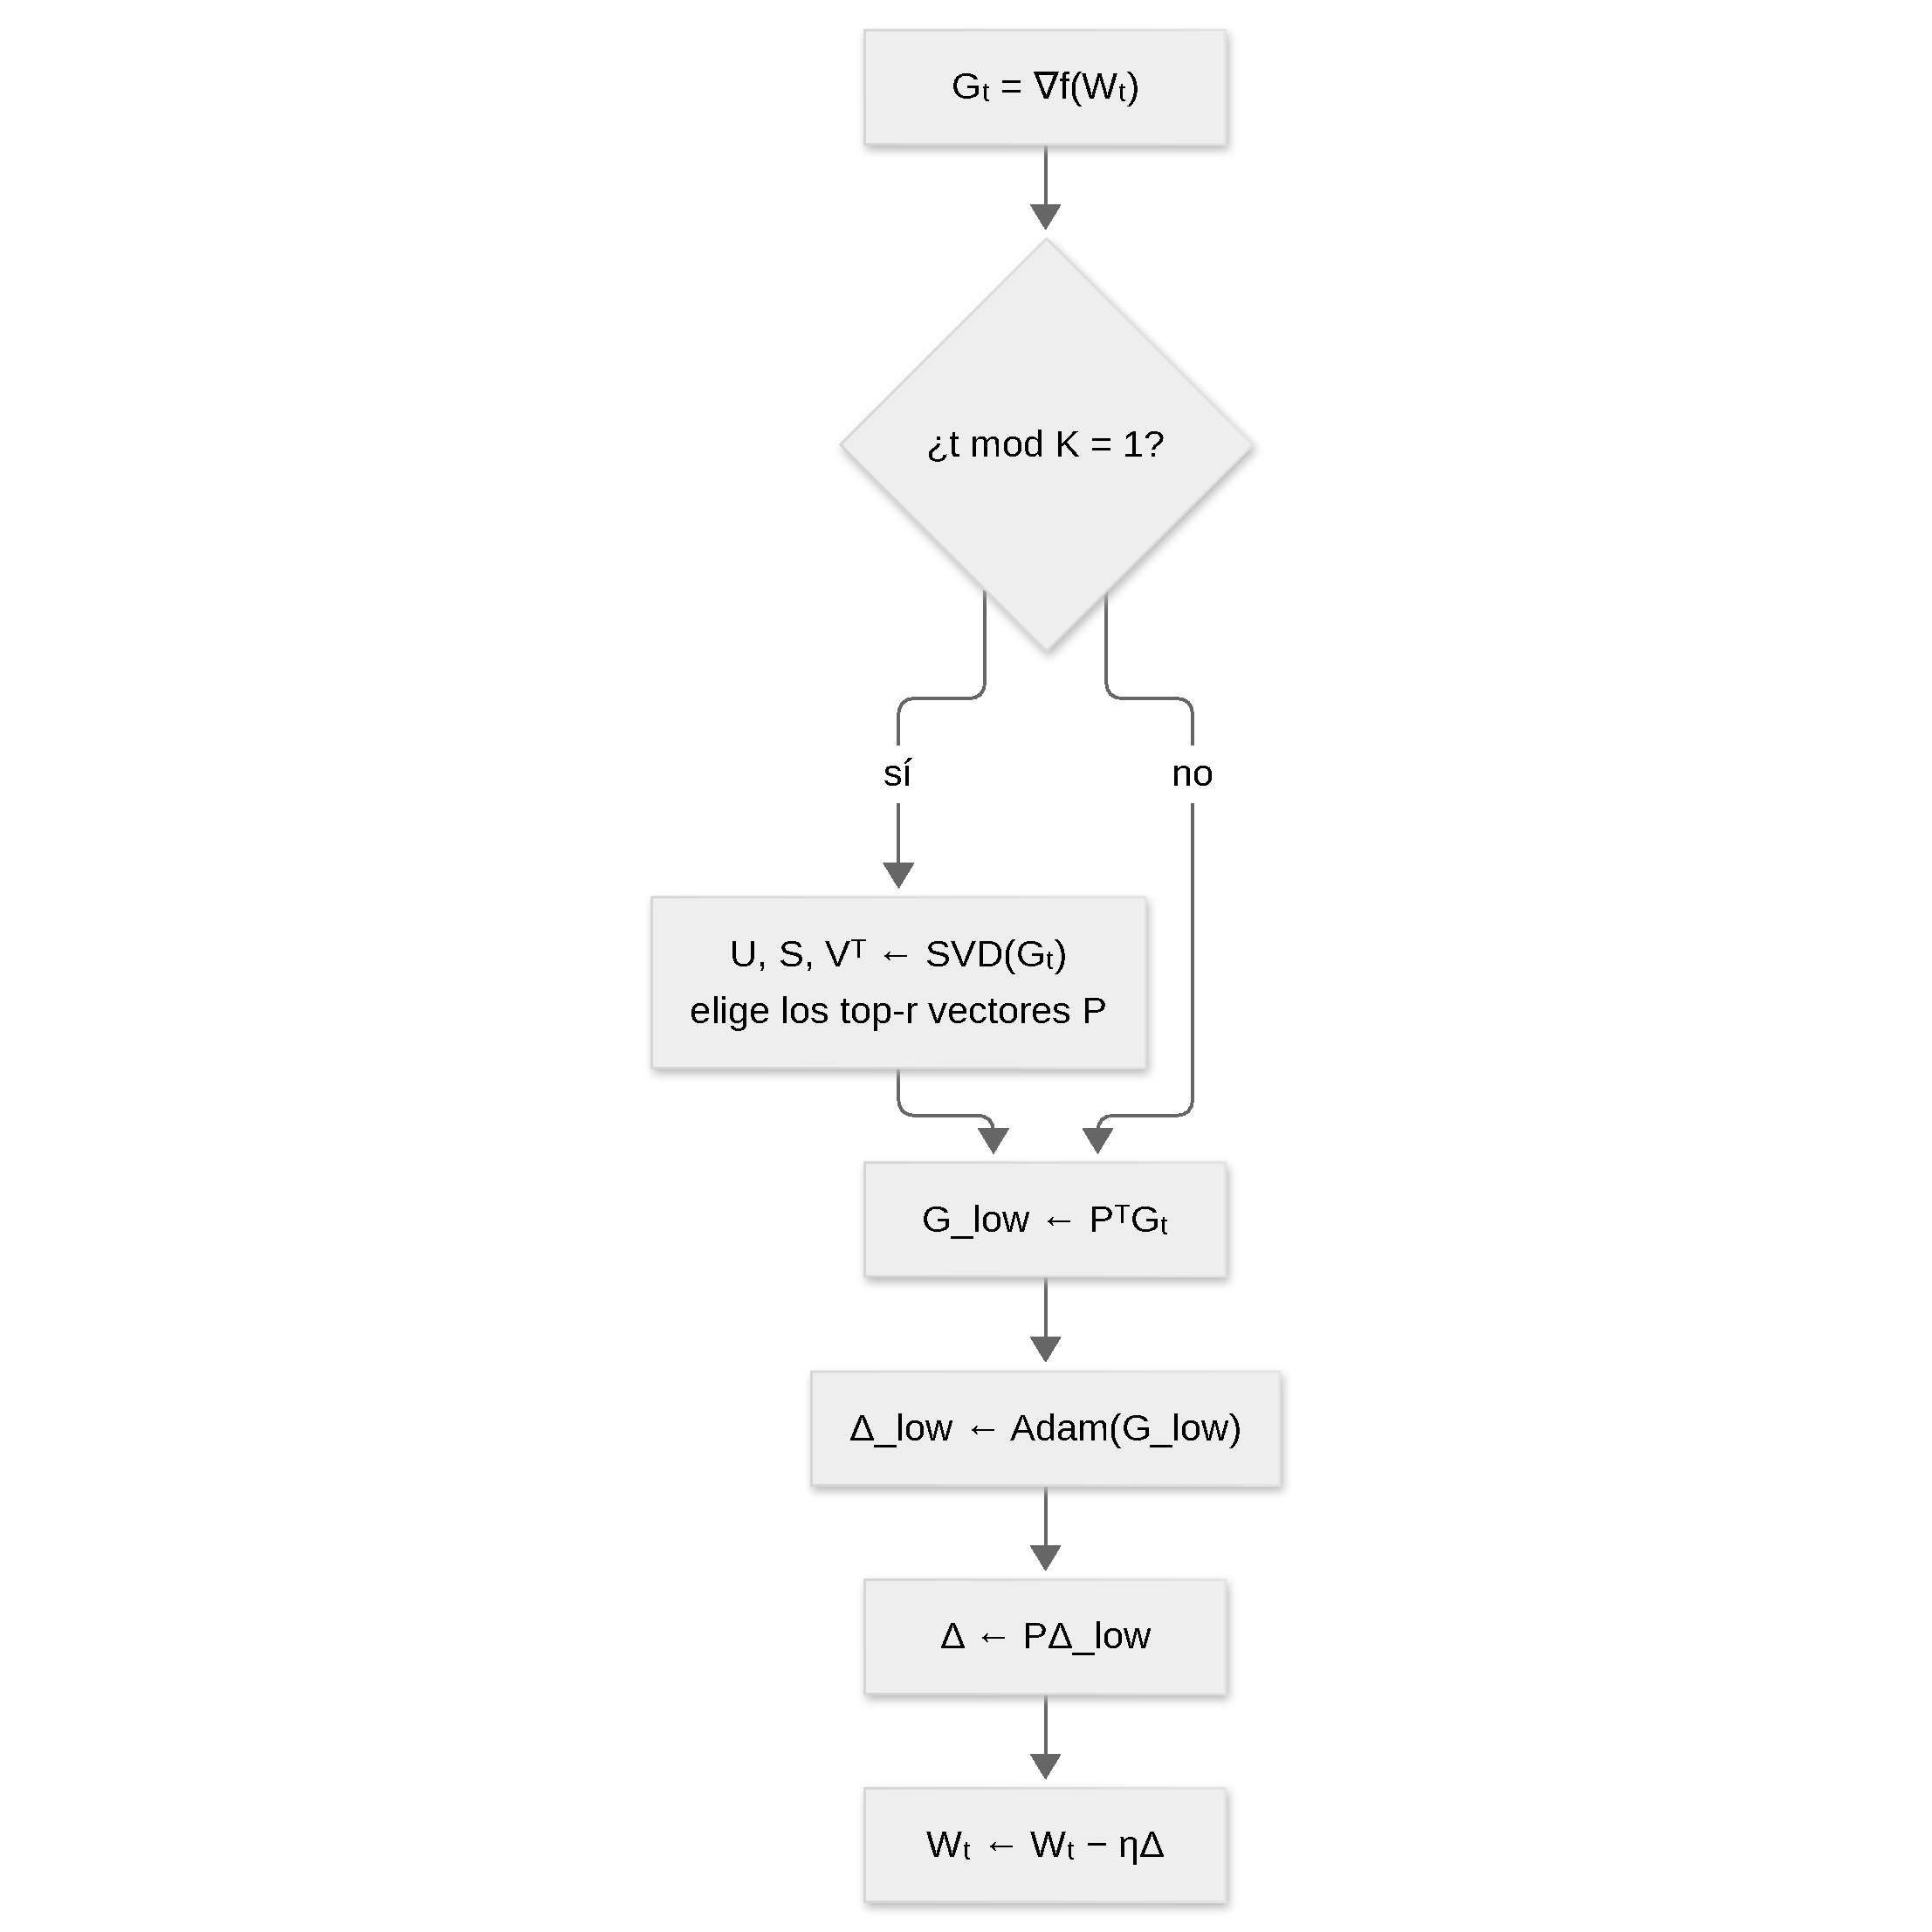
\includegraphics{../paper/figures/optimizers/galore-es.pdf}}
\caption{Flujo por paso de GaLore: proyección SVD periódica del gradiente a un subespacio de bajo rango, Adam en ese subespacio y reconstrucción.}
\label{fig:opt-galore}
\end{figure}
GaLore proyecta gradientes 2D en un subespacio de bajo rango antes de la optimización, reduciendo la memoria del estado del optimizador mientras mantiene el escalado adaptativo del paso. Para una matriz de parámetros 2D $W \in \mathbb{R}^{m \times n}$:
\begin{align}
U, S, V &= \text{SVD}(G_t) \quad\text{(calcular descomposición singular)} \\
P &\in \mathbb{R}^{n \times r} \quad\text{o} \quad P^\top \in \mathbb{R}^{r \times m} \quad\text{(seleccionar los $r$ vectores singulares superiores)} \\
G_{\text{low}} &= P^\top G_t \quad\text{(proyectar al espacio de bajo rango)} \\
\Delta_{\text{low}} &= \text{Adam}(G_{\text{low}}) \quad\text{(optimizar en el espacio comprimido)} \\
\Delta &= P \Delta_{\text{low}} \quad\text{(reconstruir en el espacio original)}
\end{align}
Al proyectar en un subespacio de rango $r$ (típicamente $r \ll \min(m,n)$), el estado del optimizador se reduce de $O(mn)$ a $O(r(m+n))$ para parámetros 2D. Este enfoque complementario de ahorro de memoria es especialmente relevante cuando el modelo es demasiado grande para el estado completo del optimizador.

\begin{algorithm}[H]
\caption{GaLore (Gradient Low-Rank Projection)}
\label{alg:galore}
\begin{algorithmic}[1]
\Require Matriz de parámetros 2D $W \in \mathbb{R}^{m \times n}$, tasa de aprendizaje $\eta$, rango $r \ll \min(m,n)$
\Ensure Parámetros actualizados $\theta_T$
\State Inicializar: Estado de Adam en el espacio de bajo rango (si es variante de rango 2)
\For{$t = 1, 2, \ldots, T$}
    \State $G_t \gets \nabla f(W_t)$
    \If{$t \mod K = 1$}  \Comment{SVD periódico}
        \State $U_t, S_t, V_t^\top \gets \text{SVD}(G_t)$ (completa o delgada)
        \State Seleccionar proyección: $P \gets U_t[:, :r]$ o $P \gets V_t[:, :r]$
    \EndIf
    \State Proyectar gradiente: $G_{\text{low}} \gets P^\top G_t$ (o $G_t P^\top$ para proyección derecha)
    \State Ejecutar Adam en bajo rango: $\Delta_{\text{low}} \gets \text{Adam}(G_{\text{low}})$
    \State Reconstruir en espacio original: $\Delta \gets P \Delta_{\text{low}}$ (o $\Delta_{\text{low}} P^\top$)
    \State $W_t \gets W_t - \eta \Delta$
\EndFor
\Return $\theta_T$
\end{algorithmic}
\end{algorithm}

\paragraph{Contras.}
\begin{itemize}[leftmargin=*]
\item El SVD periódico añade cómputo e introduce un intervalo de actualización de la proyección que ajustar.
\item La proyección de bajo rango puede descartar información del gradiente.
\end{itemize}

\paragraph{Ventajas.}
\begin{itemize}[leftmargin=*]
\item El estado del optimizador se reduce de $O(mn)$ a $O(r(m+n))$ para parámetros 2D.
\item Funciona sinérgicamente con otras técnicas y ha mostrado resultados sólidos en modelos de miles de millones de parámetros.
\end{itemize}

\paragraph{APOLLO, APOLLO-Mini, y Q-APOLLO.}
\begin{figure}[H]
\centering
\fitfigure{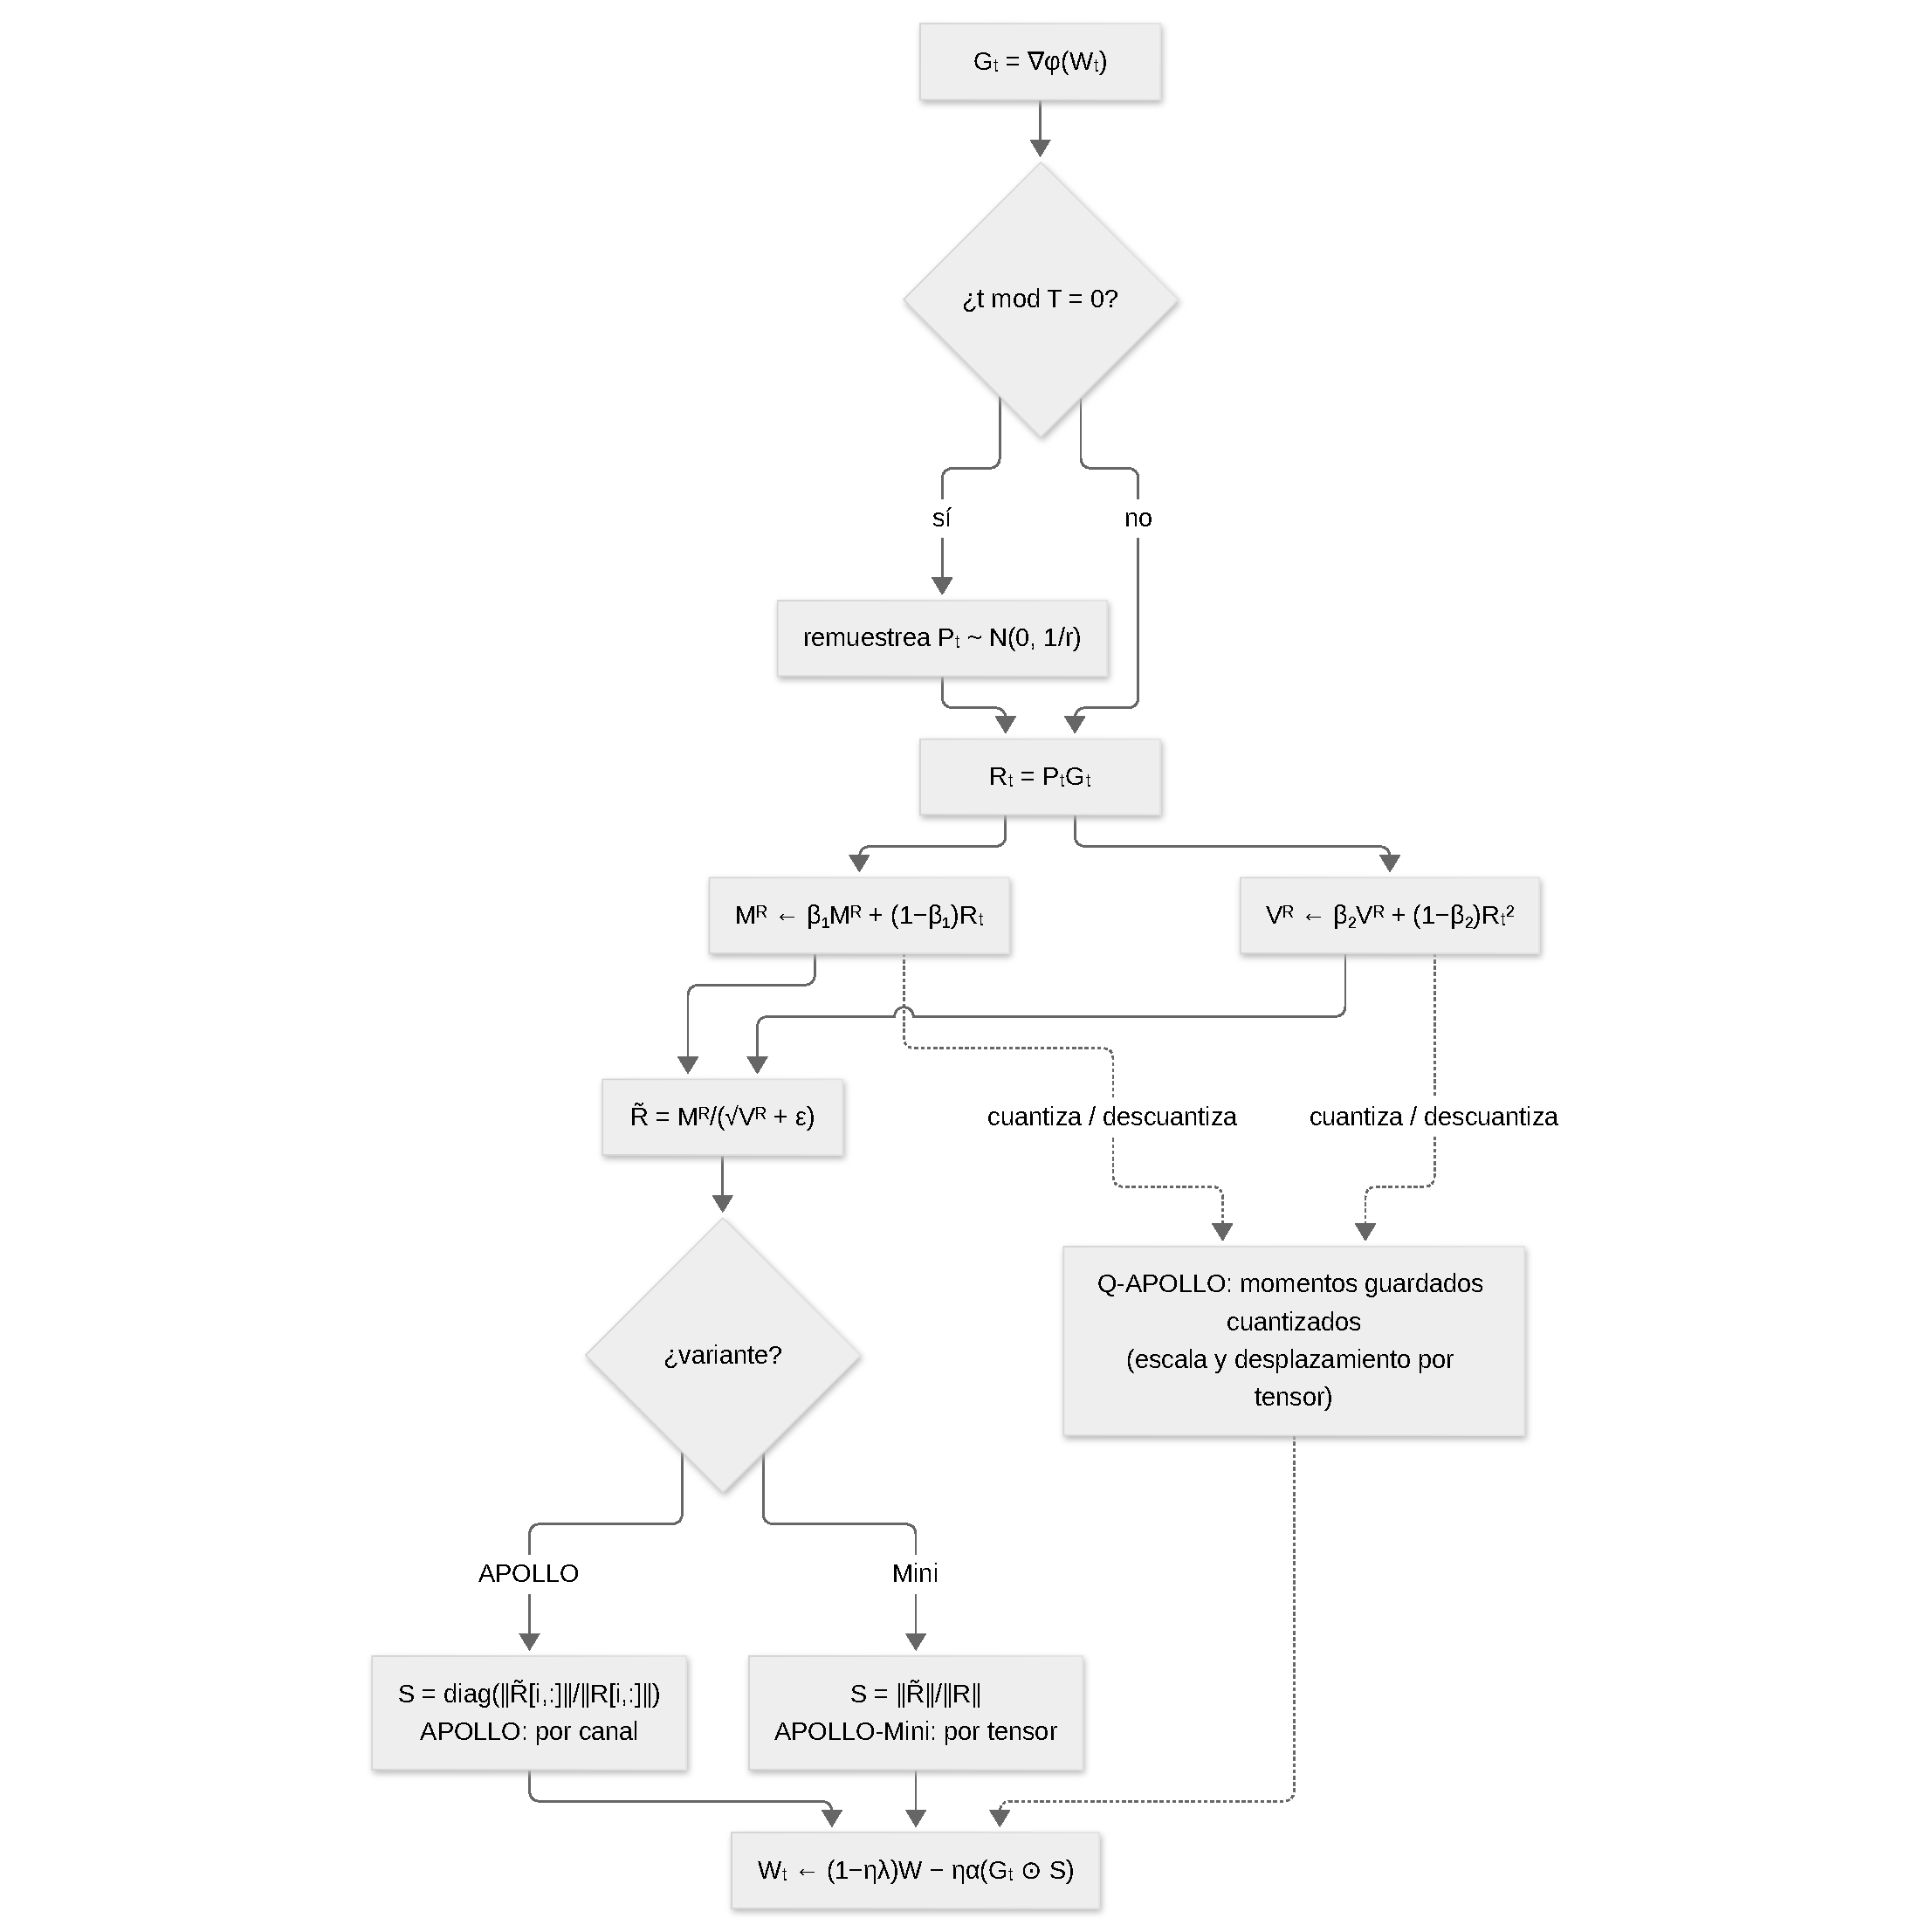
\includegraphics{../paper/figures/optimizers/apollo-es.pdf}}
\caption{Flujo por paso de la familia APOLLO: momentos proyectados gaussianos, escalado estructurado del gradiente (por canales en APOLLO, escalar en APOLLO-Mini) y estado cuantizado en Q-APOLLO.}
\label{fig:opt-apollo}
\end{figure}
La familia APOLLO \citep{zhu2025apollosgdlikememoryadamwlevel} parte de la observación de que el denominador elemento a elemento de AdamW puede \textbf{transformarse en una actualización estructurada de la tasa de aprendizaje}. En lugar de almacenar momentos densos para cada entrada de parámetro, APOLLO proyecta un gradiente matricial $G_t \in \mathbb{R}^{m \times n}$ en un subespacio aleatorio compacto y rastrea momentos estilo Adam allí:
\begin{align}
R_t &= P_t G_t \quad\text{o}\quad R_t = G_t P_t^\top \\
M_t^R &= \beta_1 M_{t-1}^R + (1-\beta_1)R_t \\
V_t^R &= \beta_2 V_{t-1}^R + (1-\beta_2)R_t^2 \\
\widetilde{R}_t &= \frac{M_t^R}{\sqrt{V_t^R}+\epsilon}
\end{align}
El estado proyectado \emph{no} se expande de vuelta a una actualización densa de bajo rango como en los métodos basados en SVD. En su lugar, APOLLO estima un tensor de escalado estructurado $S_t$ en el espacio original. En la variante estándar de APOLLO, ese escalado es \textbf{por canales}: cada fila o canal recibe su propia razón de norma. En APOLLO-Mini, el escalado se reduce a un único escalar \textbf{por tensor}, correspondiente al caso extremo de rango 1 descrito en el artículo. La actualización de parámetros resultante es, por tanto, similar a Adam en adaptación pero mucho más cercana a SGD en costo de estado:
\[
W_t \gets (1-\eta\lambda)W_{t-1} - \eta\,\alpha\,(G_t \odot S_t)
\]
donde $\alpha$ es el factor de escala adicional usado para estabilizar variantes altamente comprimidas.

\begin{algorithm}[H]
\caption{APOLLO / APOLLO-Mini Escalado de Gradiente Estructurado}
\label{alg:apollo-family}
\begin{algorithmic}[1]
\Require Matriz de pesos $W \in \mathbb{R}^{m \times n}$ con $m \le n$, tasa de aprendizaje $\eta$, factor de escala $\alpha$, tasas de decaimiento $(\beta_1, \beta_2)$, decaimiento de pesos $\lambda$, rango $r$, intervalo de actualización de proyección $T$
\Ensure Parámetros actualizados $W_T$
\State Inicializar momentos proyectados: $M^R \gets 0$, $V^R \gets 0$, paso $t \gets 0$
\Repeat
    \State Calcular gradiente: $G_t \gets \nabla_W \phi(W_t)$
    \If{$t \bmod T = 0$}
        \State Muestrear proyector gaussiano $P_t \sim \mathcal{N}(0, 1/r)$ con una semilla nueva
    \EndIf
    \State Proyectar gradiente: $R_t \gets P_t G_t$ \Comment{o $G_t P_t^\top$ según la disposición}
    \State Actualizar momentos proyectados AdamW: $M_t^R, V_t^R \gets \text{AdamWState}(R_t; \beta_1, \beta_2)$
    \State Normalizar estado proyectado: $\widetilde{R}_t \gets M_t^R / (\sqrt{V_t^R}+\epsilon)$
    \If{APOLLO}
        \State $S_t \gets \operatorname{diag}(s_1^R, \ldots, s_m^R)$, donde $s_i^R = \|\widetilde{R}_t[i,:]\|_2 / \|R_t[i,:]\|_2$
    \Else
        \State $S_t \gets s_t^R$, donde $s_t^R = \|\widetilde{R}_t\|_2 / \|R_t\|_2$
    \EndIf
    \State Actualizar pesos: $W_t \gets (1-\eta\lambda)W_{t-1} - \eta\,\alpha\,(G_t \odot S_t)$
    \State $t \gets t+1$
\Until{convergencia}
\end{algorithmic}
\end{algorithm}

\paragraph{Contras.}
\begin{itemize}[leftmargin=*]
\item El escalado estructurado es una aproximación más gruesa del denominador elemento a elemento de AdamW.
\item Las proyecciones deben refrescarse periódicamente y rangos muy pequeños hacen que el escalado sea ruidoso.
\end{itemize}

\paragraph{Ventajas.}
\begin{itemize}[leftmargin=*]
\item Reemplaza el SVD repetido con proyección aleatoria gaussiana refrescada periódicamente, de modo que el costo de sistemas es multiplicación de matrices ordinaria en lugar de descomposición espectral.
\item Inusualmente tolerante a la compresión extrema: incluso APOLLO-Mini, que solo mantiene estado auxiliar de rango 1, sigue siendo competitivo o mejor que AdamW mientras se acerca al costo de memoria de SGD.
\end{itemize}

\paragraph{APOLLO-Mini.}
APOLLO-Mini es el miembro de la familia optimizado para \textbf{eficiencia de memoria extrema}. El artículo lo motiva argumentando que, en un espacio compacto de rango 1, el escalado por canales se vuelve demasiado ruidoso, por lo que la actualización se simplifica aún más a un único escalar por tensor. La pérdida de granularidad se compensa parcialmente con el factor de escala explícito $\alpha$ (el artículo discute valores como $128$ en este régimen), proporcionando un punto útil en la frontera de Pareto de optimización: estado muy pequeño, sin sobrecarga de SVD, y aún un comportamiento sólido en preentrenamiento.

\paragraph{Contras.}
\begin{itemize}[leftmargin=*]
\item Un único escalar por tensor pierde granularidad por canales, y el estado de rango 1 puede ser ruidoso.
\item Depende del factor de escala adicional $\alpha$ (e.g., $128$) para mantenerse estable.
\end{itemize}

\paragraph{Ventajas.}
\begin{itemize}[leftmargin=*]
\item El estado más pequeño de la familia APOLLO, sin sobrecarga de SVD.
\item Comportamiento sólido en preentrenamiento con un costo de memoria cercano a SGD.
\end{itemize}

\paragraph{Q-APOLLO.}
El artículo de APOLLO también enfatiza que la familia se combina naturalmente con \textbf{cuantización} para entrenamiento con memoria ultra-baja. Este repositorio convierte esa observación de sistemas en una variante concreta del optimizador, \texttt{q\_apollo}. En la implementación, los momentos de primer y segundo orden de bajo rango de APOLLO se almacenan en forma cuantizada junto con escalas y desplazamientos por tensor, y se descuantizan solo cuando es necesario para el siguiente paso. Q-APOLLO preserva, por tanto, la lógica de gradiente proyectado de APOLLO mientras reduce la precisión del estado restante del optimizador.

\paragraph{Contras.}
\begin{itemize}[leftmargin=*]
\item Los momentos cuantizados introducen error de aproximación y sobrecarga de descuantización.
\item Requiere gestionar escalas y desplazamientos por tensor.
\end{itemize}

\paragraph{Ventajas.}
\begin{itemize}[leftmargin=*]
\item Reduce el estado restante del optimizador a precisión ultra baja.
\item Miembro más agresivo en ahorro de memoria de la pila local, preservando la lógica de gradiente proyectado de APOLLO.
\end{itemize}

\paragraph{AdamPM (Adam con momentos agrupados).}
AdamPM~\citep{ji_adampm_2026} es una \textbf{modificación mínima y agnóstica al
modelo de Adam}: conserva el primer momento por elemento y comprime únicamente
el segundo momento mediante el \textbf{promedio por grupo de entradas
adyacentes} a lo largo de cada fila (el valor por defecto, siendo las filas las
características de salida) o de cada columna (la variante \emph{AdamPM-col} del
artículo). Para una matriz de pesos $W \in \mathbb{R}^{m \times n}$ y un tamaño
de grupo $s$, cada fila se particiona en $q = \lceil n/s \rceil$ grupos, el
gradiente al cuadrado se promedia dentro de cada grupo \emph{antes} de la media
móvil exponencial, y solo se persiste el estadístico comprimido
$\bar{V}_t \in \mathbb{R}^{m \times q}$:
\begin{align}
M_t &= \beta_1 M_{t-1} + (1-\beta_1)\, G_t
     && \text{(primer momento, por elemento, Ec.~1)} \\
\bar{S}_t &= \frac{1}{s}\sum_{k=1}^{s}
     \mathrm{reshape}(G_t \odot G_t,\, m, q, s)[:,:,k]
     && \text{(medias por grupo, Ec.~2)} \\
\bar{V}_t &= \beta_2 \bar{V}_{t-1} + (1-\beta_2)\, \bar{S}_t
     && \text{(EMA comprimida del segundo momento, Ec.~3)} \\
W_t &= W_{t-1} - \eta_t \,
     \frac{M_t/(1-\beta_1^t)}
          {\sqrt{\hat{\bar{V}}_t \otimes \mathbf{1}_{1\times s}} + \epsilon},
\qquad \hat{\bar{V}}_t = \frac{\bar{V}_t}{1-\beta_2^t}
     && \text{(actualización, Ec.~4)}
\end{align}
Cuando $n$ no es divisible por $s$, el último grupo se rellena con su propia
media, de modo que su estadístico promedia solo las entradas que realmente
contiene; $s{=}1$ recupera Adam exactamente y $s \ge n$ colapsa cada fila (o
columna) a un escalar, el límite \emph{AdamPM-inf} del artículo. AdamPM agrupa
los segundos momentos de \textbf{todas} las matrices de pesos---embeddings, la
cabeza LM, atención y pesos MLP---y trata los parámetros unidimensionales, como
las escalas RMSNorm, como matrices de una sola fila o de una sola columna, de
modo que ningún grupo de parámetros queda en una ruta de respaldo. El estado
persistente es de $mn(1+1/s)$ elementos frente a los $2mn$ de Adam.

\begin{algorithm}[H]
\caption{AdamPM (Adam con momentos agrupados)}
\label{alg:adampm}
\begin{algorithmic}[1]
\Require Parámetros iniciales $W_0 \in \mathbb{R}^{m\times n}$, pasos $T$, tamaño de grupo $s$, tasa de aprendizaje $\eta_t$, tasas de decaimiento $\beta_1, \beta_2$, constante de estabilidad $\epsilon$
\Ensure Parámetros actualizados $W_T$
\State $t \gets 0$; \ $q \gets \lceil n/s \rceil$ \Comment{Número de grupos por fila}
\State $M_0 \gets \mathbf{0}_{m\times n}$; \ $\bar{V}_0 \gets \mathbf{0}_{m\times q}$ \Comment{Primer momento y segundo momento comprimido}
\Repeat
    \State $t \gets t + 1$
    \State $G_t \gets \nabla_W \mathcal{L}(W_{t-1})$ \Comment{Gradiente}
    \State $M_t \gets \beta_1 M_{t-1} + (1-\beta_1) G_t$ \Comment{EMA del primer momento (Ec.~1)}
    \State $\bar{S}_t \gets \operatorname{mean}_{k}\big(\mathrm{reshape}(G_t \odot G_t, m, q, s)[:,:,k]\big)$ \Comment{Medias por grupo (Ec.~2)}
    \State $\bar{V}_t \gets \beta_2 \bar{V}_{t-1} + (1-\beta_2) \bar{S}_t$ \Comment{EMA comprimida del segundo momento (Ec.~3)}
    \State $\hat{M}_t \gets M_t/(1-\beta_1^t)$; \ $\hat{\bar{V}}_t \gets \bar{V}_t/(1-\beta_2^t)$ \Comment{Correcciones de sesgo}
    \State difundir $\hat{\bar{V}}_t$ sobre cada grupo \Comment{Producto de Kronecker con $\mathbf{1}_{1\times s}$}
    \State $W_t \gets W_{t-1} - \eta_t \hat{M}_t / (\sqrt{\hat{\bar{V}}_t} + \epsilon)$ \Comment{Actualización (Ec.~4)}
\Until{$t = T$ o convergencia}
\Return $W_t$
\end{algorithmic}
\end{algorithm}

Empíricamente, AdamPM iguala a un Adam cuidadosamente ajustado en el
preentrenamiento de LLaMA de 60M a 1.3B parámetros mientras recorta la memoria
del segundo momento un 87,5\,\% ($s{=}8$) y hasta un 93,75\,\% ($s{=}16$), con
el mismo patrón en el ajuste fino de RoBERTa-base sobre GLUE y en el
entrenamiento supervisado de TinyLLaVA-1B; los tamaños de grupo entre 2 y 8 se
reportan como robustos, y tres o cinco---no solo potencias de dos---funcionan
porque el último grupo incompleto se promedia sobre sus propias entradas. El
Teorema~3.1 ofrece una cota de estacionariedad independiente del tamaño de
grupo $s$ y, bajo una condición de ruido relativo, AdamPM alcanza la misma tasa
$\mathcal{O}(\log T/\sqrt{T})$ que Adam. El Algoritmo~1 del artículo no define
weight decay; esta implementación aplica el decaimiento desacoplado
\texttt{wd\_*} del repositorio antes de la actualización adaptativa, y los
sufijos compartidos \texttt{betas}/\texttt{eps} por grupo parametrizan las
correcciones de sesgo y el denominador.

\paragraph{Contras.}
\begin{itemize}[leftmargin=*]
\item El precondicionador diagonal se vuelve más grueso a medida que crece $s$;
      el límite AdamPM-inf del artículo muestra una pérdida de perplejidad
      medible en 350M y 1.3B.
\item El ahorro cubre solo el estado del optimizador: el primer momento
      permanece a tamaño completo, así que la memoria del optimizador es
      $1+1/s$ la de Adam, no $1/s$.
\item El pooling es unidimensional (filas o columnas); los grupos
      bidimensionales y el pooling selectivo por capa quedan sin explorar
      (limitaciones del artículo).
\end{itemize}

\paragraph{Ventajas.}
\begin{itemize}[leftmargin=*]
\item Aproximadamente la mitad de la memoria de estado del optimizador con el
      valor por defecto $s{=}8$ (segundo momento a $1/8$), con perplejidad
      al nivel de Adam hasta 1.3B parámetros y sobrecarga por paso
      despreciable---sin SVD, sin proyección, sin estado extra.
\item Hereda directamente la tasa de aprendizaje y las tasas de decaimiento de
      Adam, de modo que los presets de Adam se transfieren sin reajuste y
      $\beta_1{=}0.9$, $\beta_2{=}0.95$ coinciden con los valores por defecto
      del repositorio.
\item Agnóstico al modelo y aplicable uniformemente a todos los grupos de
      parámetros; las actualizaciones precondicionadas se parecen más a las de
      Adam a medida que crece la escala del modelo.
\end{itemize}

\paragraph{Anon (Adaptivity Non-restricted Optimizer with Novel convergence technique).}
\begin{figure}[H]
\centering
\fitfigure{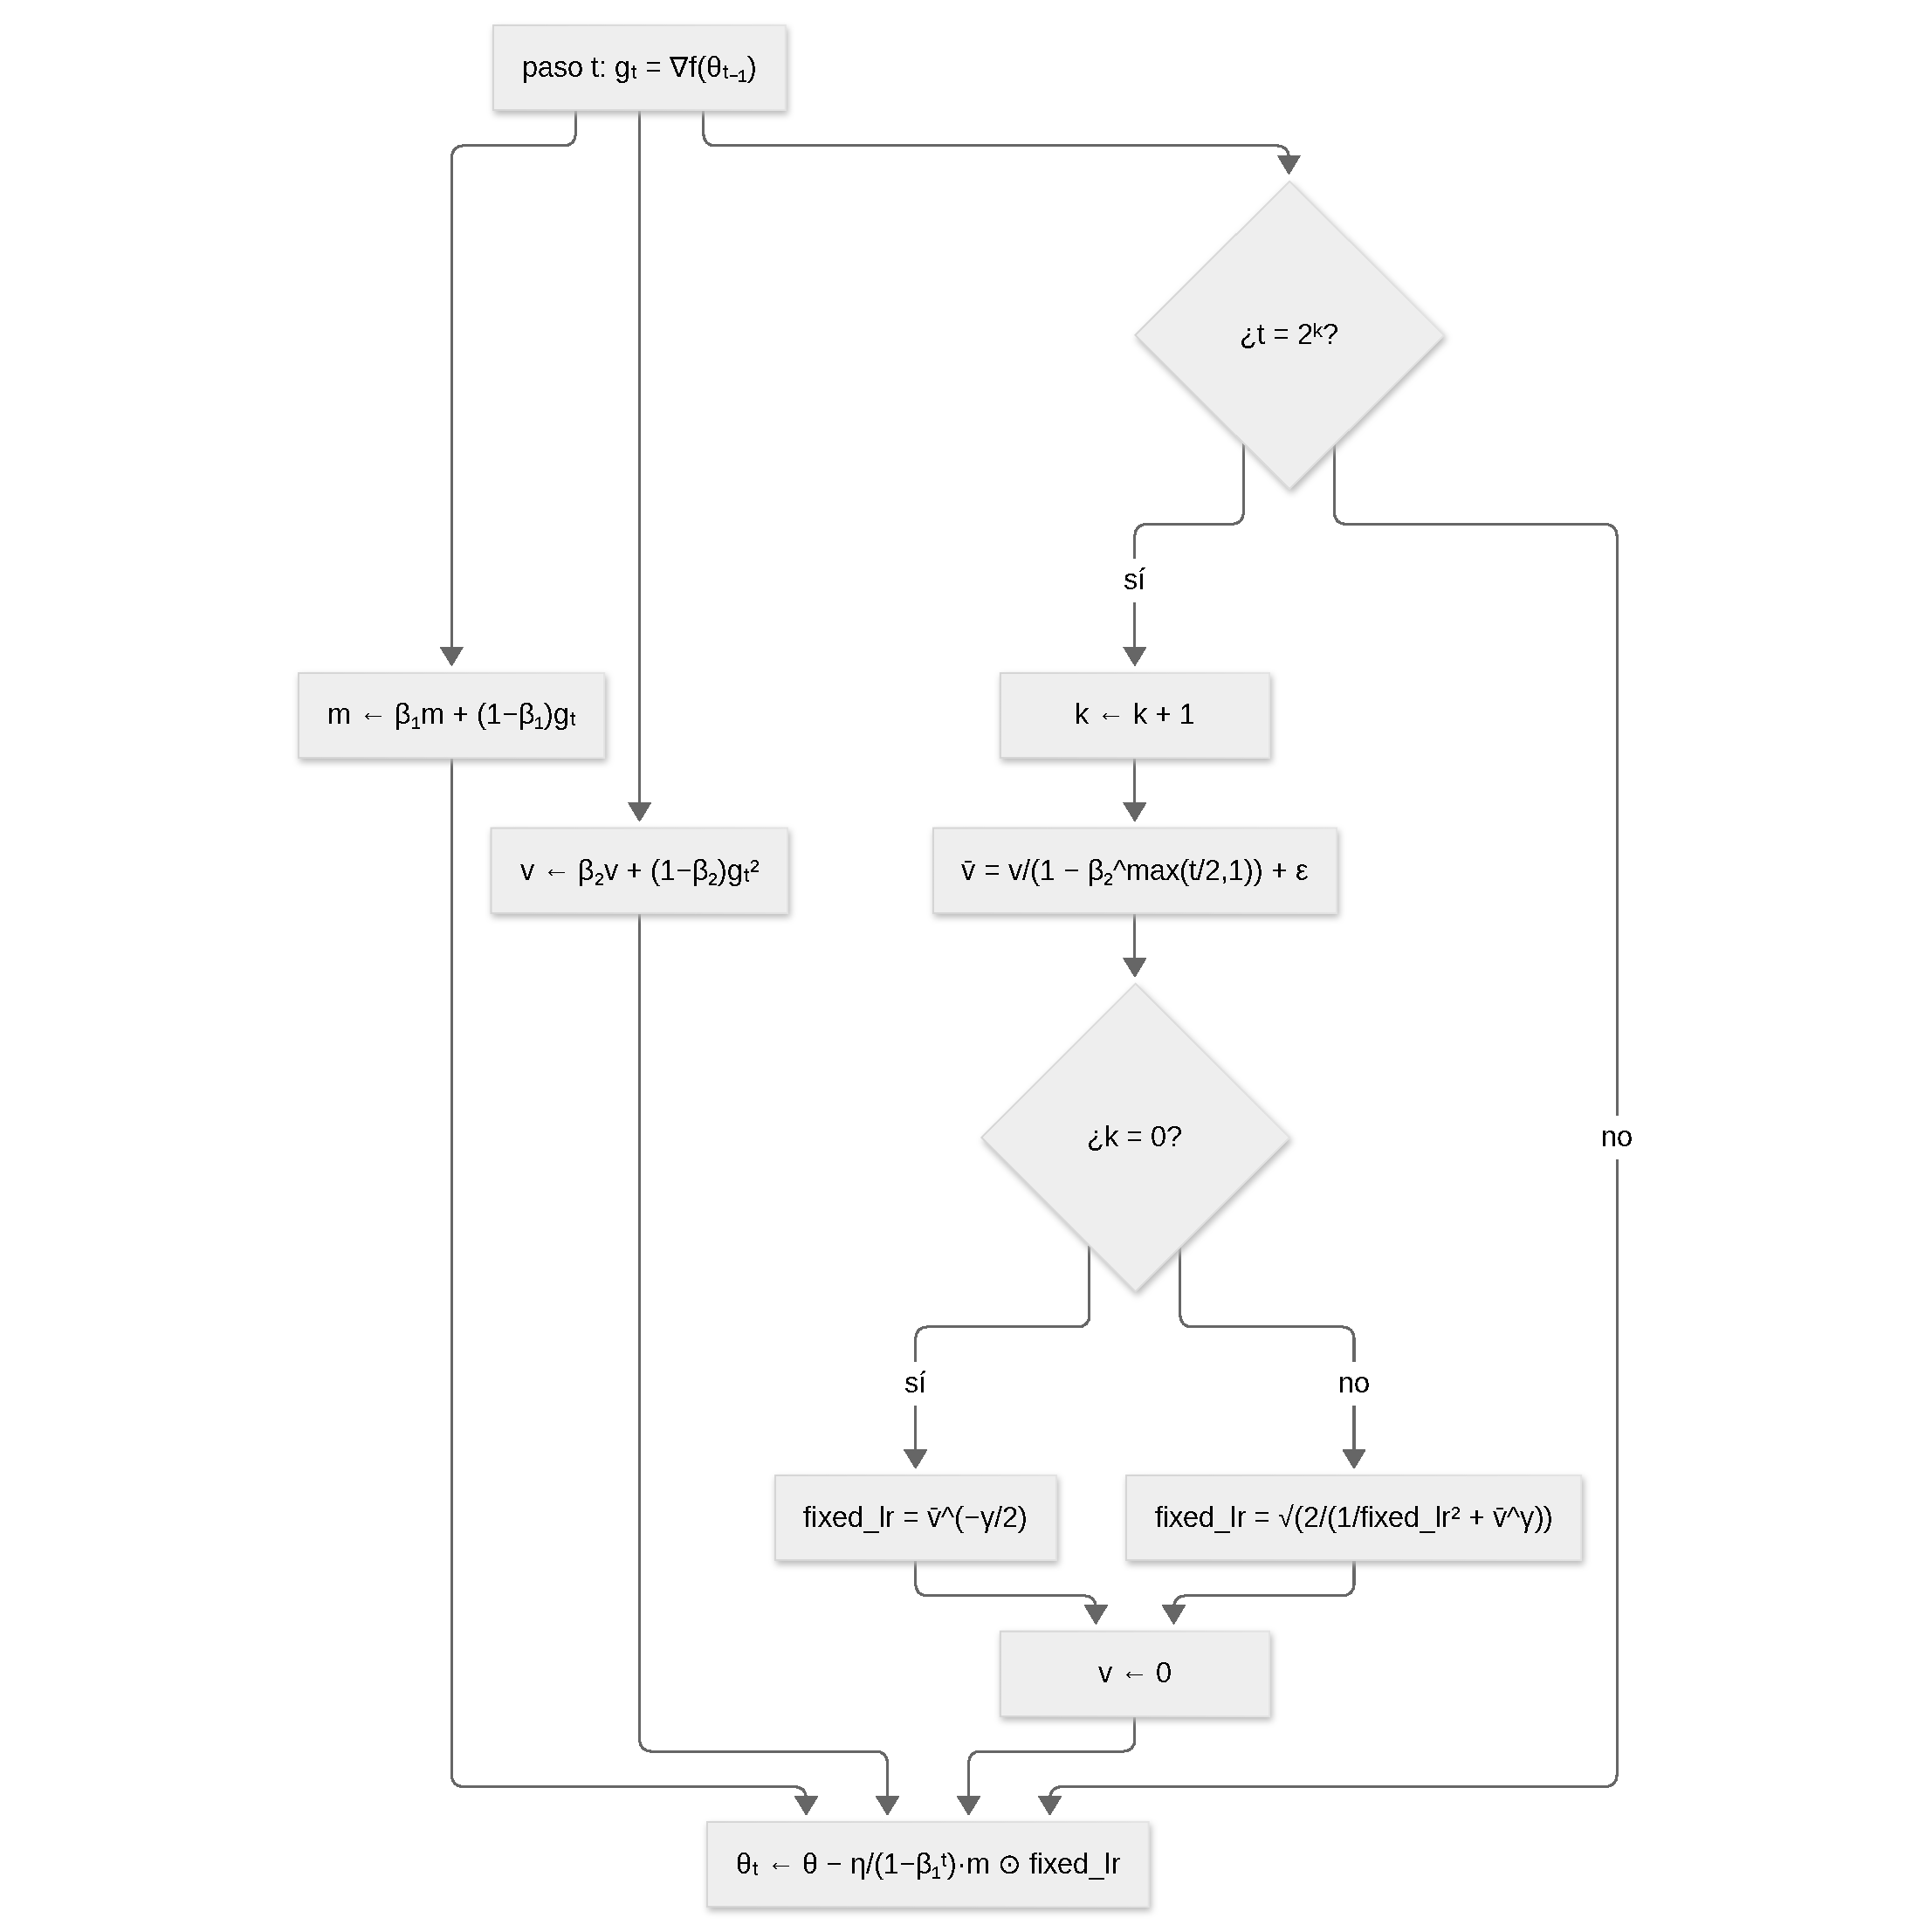
\includegraphics{../paper/figures/optimizers/anon-es.pdf}}
\caption{Flujo por paso de Anon: el precondicionador IDU refrescado en potencias de dos, con adaptividad ajustable $\gamma$ y una actualización de momentum con corrección de sesgo.}
\label{fig:opt-anon}
\end{figure}
Anon \citep{anon2026anon} introduce adaptividad ajustable continuamente mediante un único parámetro $\gamma \in \mathbb{R}$, cerrando la brecha entre comportamientos tipo SGD ($\gamma=0$) y tipo Adam ($\gamma=1$), y extrapolando más allá de ambos. La innovación central es el mecanismo Incremental Delay Update (IDU), que permite convergencia estable a través de todo el espectro de adaptividad de valores reales:

\begin{align}
m_t &= \beta_1 m_{t-1} + (1-\beta_1) g_t \quad\text{(momento de primer orden)}\\
v_t &= \beta_2 v_{t-1} + (1-\beta_2) g_t^2 \quad\text{(momento de segundo orden)}\\
\bar{v}_t &= \frac{v_t}{1-\beta_2^{\max(t,1)}} + \epsilon \quad\text{(momento de segundo orden con corrección de sesgo)}\\
\text{fixed\_lr}_k &= \begin{cases}
\bar{v}_k^{-\gamma/2} & \text{si } k = 0 \\
\sqrt{2 / \left(\frac{1}{\text{fixed\_lr}_{k-1}^2} + \bar{v}_k^\gamma\right)} & \text{si } k > 0
\end{cases}\\
\theta_{t+1} &= \theta_t - \frac{\eta}{1-\beta_1^t} \cdot m_t \odot \text{fixed\_lr}_{\lfloor\log_2 t\rfloor}
\end{align}

A diferencia de los optimizadores adaptativos estándar, IDU actualiza el precondicionador solo en potencias de dos ($t = 2^k$), acumulando estadísticas de gradiente entre actualizaciones y agregándolas recursivamente. Este acumulador suave y multiescala evita el seguimiento estricto del máximo de AMSGrad mientras estabiliza demostrablemente la convergencia para cualquier $\gamma \in \mathbb{R}$. El parámetro $\gamma$ controla directamente la adaptividad: $\gamma > 1$ acelera la salida de puntos de silla (favorable para arquitecturas complejas), $\gamma = 1$ recupera el comportamiento tipo Adam, $\gamma = 0$ produce escalado tipo SGD, y $\gamma < 0$ se sesga hacia mínimos más planos (beneficioso para arquitecturas clásicas como CNNs).

\begin{algorithm}[H]
\caption{Anon (Adaptivity Non-restricted Optimizer con IDU)}
\label{alg:anon}
\begin{algorithmic}[1]
\Require Parámetros iniciales $\theta_0$, tasa de aprendizaje $\eta$, $\beta_1, \beta_2$, tolerancia $\epsilon$, adaptividad $\gamma \in \mathbb{R}$
\Ensure Parámetros actualizados $\theta_T$
\State Inicializar: $m \gets 0$, $v \gets 0$, $fixed\_lr \gets 0$, paso $t \gets 0$, contador IDU $k \gets -1$
\For{$t = 1, 2, \ldots, T$}
    \State $g_t \gets \nabla f(\theta_{t-1})$
    \State $m \gets \beta_1 m + (1-\beta_1) g_t$
    \State $v \gets \beta_2 v + (1-\beta_2) g_t^2$
    \If{$t = 2^k$}
        \State $k \gets k+1$
        \State $\bar{v} \gets v/(1 - \beta_2^{\max(t/2,1)}) + \epsilon$
        \If{$k = 0$}
            \State fixed\_lr $\gets \bar{v}^{-\gamma/2}$
        \Else
            \State fixed\_lr $\gets \sqrt{2 / (1/\text{fixed\_lr}^2 + \bar{v}^\gamma)}$
        \EndIf
        \State $v \gets 0$
    \EndIf
    \State $\theta_t \gets \theta_{t-1} - \frac{\eta}{1-\beta_1^t} \cdot m \odot \text{fixed\_lr}$
\EndFor
\Return $\theta_T$
\end{algorithmic}
\end{algorithm}

\paragraph{Contras.}
\begin{itemize}[leftmargin=*]
\item Mantiene tres búferes de estado ($m$, $v$, fixed\_lr) y refresca el precondicionador con una programación logarítmica.
\item El parámetro de adaptividad $\gamma$ debe seleccionarse por arquitectura.
\end{itemize}

\paragraph{Ventajas.}
\begin{itemize}[leftmargin=*]
\item Misma clase de complejidad $\mathcal{O}(n)$ por paso que AdamW, con adaptividad ajustable de forma continua.
\item IDU alcanza demostrablemente regret $\mathcal{O}(\sqrt{T})$ para problemas convexos y $\mathcal{O}(\ln T/\sqrt{T})$ para entornos no convexos.
\end{itemize}

\paragraph{Prodigy (Approximating the Distance Estimate).}
\begin{figure}[H]
\centering
\fitfigure{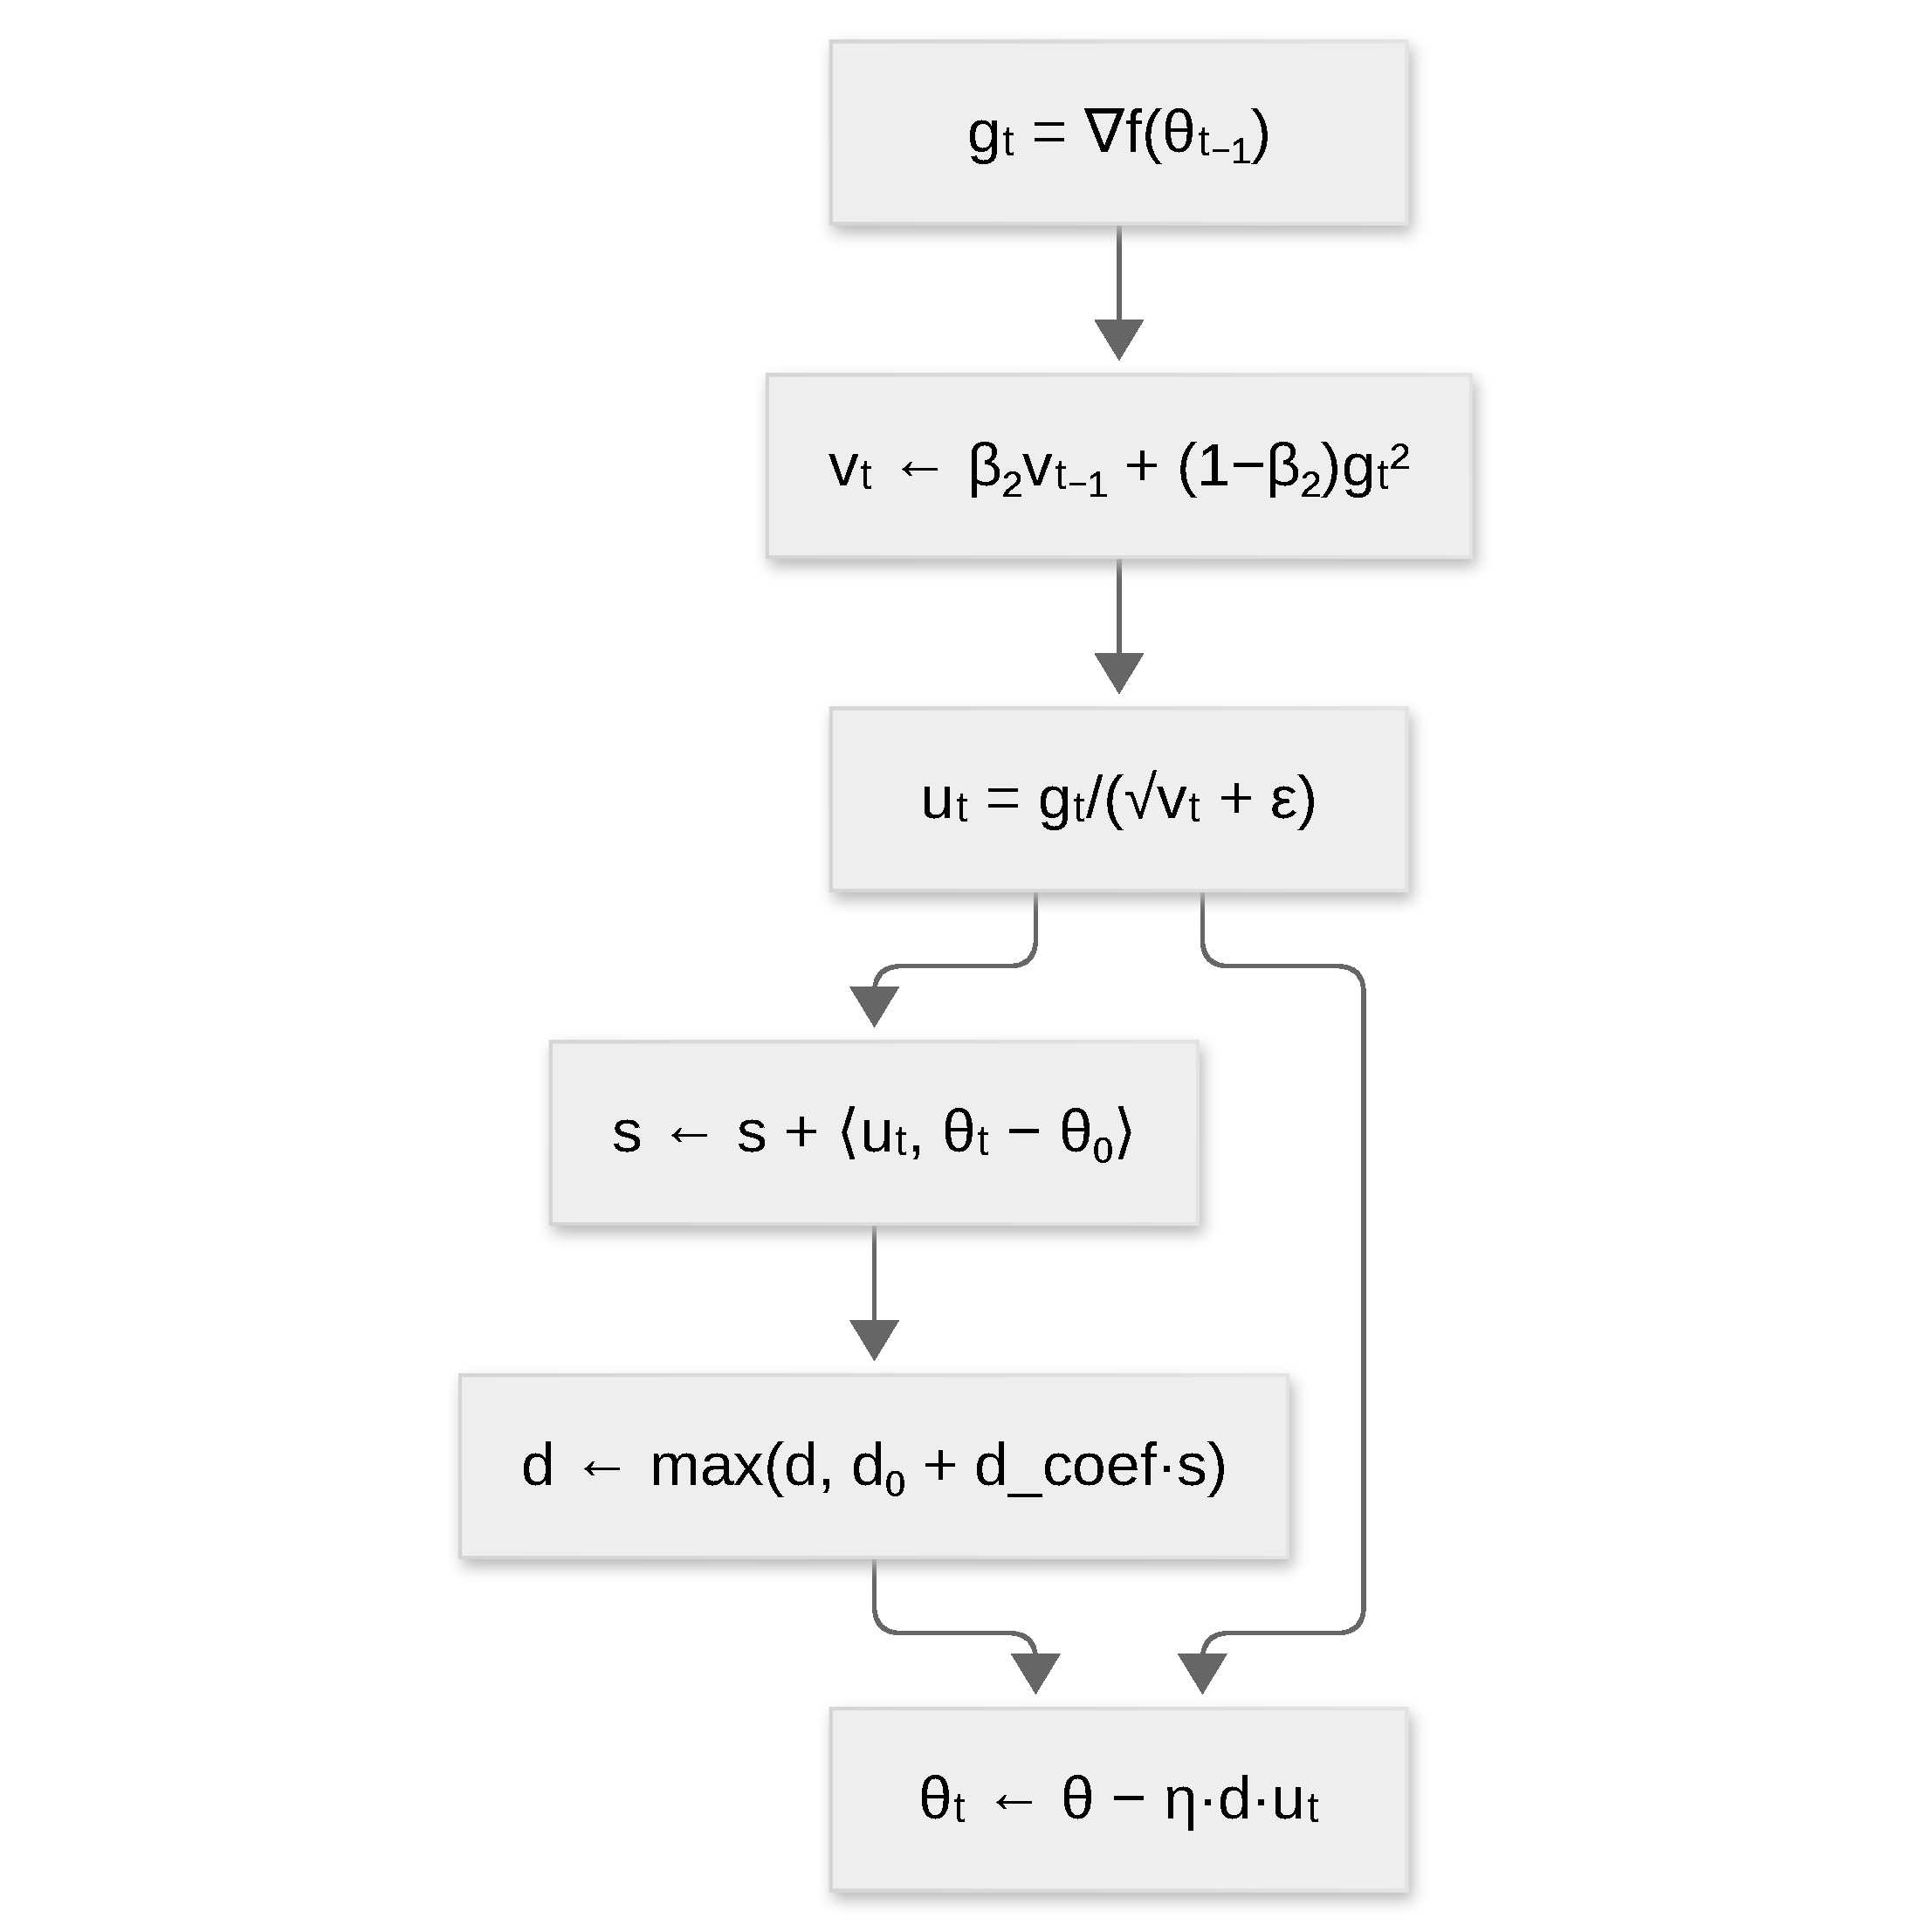
\includegraphics{../paper/figures/optimizers/prodigy-es.pdf}}
\caption{Flujo por paso de Prodigy: una estimación de distancia signada acumulativa que escala el paso adaptativo sin programación de tasa de aprendizaje.}
\label{fig:opt-prodigy}
\end{figure}
Prodigy adapta la escala efectiva del paso mediante una estadística tipo distancia acumulativa, eliminando la necesidad de ajuste explícito de la tasa de aprendizaje. El algoritmo mantiene una estimación de distancia acumulativa:
\begin{align}
u_t &= \frac{g_t}{\sqrt{v_t}+\epsilon} \quad\text{(paso adaptativo no normalizado)} \\
s_t &= s_{t-1} + \langle u_t, \theta_t - \theta_0 \rangle \quad\text{(distancia signada acumulativa)} \\
d_t &= \max(d_{t-1}, d_0 + d_{\text{coef}} \cdot s_t) \quad\text{(estimación de distancia con cota inferior)} \\
\theta_{t+1} &= \theta_t - \eta \cdot d_t \cdot u_t
\end{align}
donde $d_0$ es una cota inicial y $d_{\text{coef}}$ controla qué tan agresivamente se adapta la estimación. La estimación de distancia $d_t$ captura la magnitud combinada de gradientes pasados ponderada por el desplazamiento real de los parámetros, implementando una tasa de aprendizaje efectiva implícita.

\begin{algorithm}[H]
\caption{Prodigy (Approximating the Distance Estimate)}
\label{alg:prodigy}
\begin{algorithmic}[1]
\Require Parámetros iniciales $\theta_0$, tasa de aprendizaje $\eta$, coeficiente $d_{\text{coef}}$, distancia inicial $d_0 > 0$
\Ensure Parámetros actualizados $\theta_T$
\State Inicializar: $s \gets 0$ (distancia signada acumulativa), $d \gets d_0$
\For{$t = 1, 2, \ldots, T$}
    \State $g_t \gets \nabla f(\theta_{t-1})$
    \State $v_t \gets \beta_2 v_{t-1} + (1-\beta_2) g_t^2$ \Comment{Segundo momento}
    \State $u_t \gets g_t / (\sqrt{v_t} + \epsilon)$ \Comment{Adaptativo no normalizado}
    \State Actualizar distancia: $s \gets s + \langle u_t, \theta_t - \theta_0 \rangle$ \Comment{Distancia signada}
    \State $d \gets \max(d, d_0 + d_{\text{coef}} \cdot s)$ \Comment{Distancia con cota inferior}
    \State $\theta_t \gets \theta_{t-1} - \eta \cdot d \cdot u_t$ \Comment{Actualización escalada por distancia}
\EndFor
\Return $\theta_T$
\end{algorithmic}
\end{algorithm}

\paragraph{Contras.}
\begin{itemize}[leftmargin=*]
\item Introduce los hiperparámetros $d_0$ y $d_{\text{coef}}$ para la estimación de distancia.
\item Añade un paso de contabilidad de producto interno por iteración.
\end{itemize}

\paragraph{Ventajas.}
\begin{itemize}[leftmargin=*]
\item Elimina el ajuste y la programación explícitos de la tasa de aprendizaje.
\item Convergencia robusta en distintas escalas de problemas y tamaños de lote.
\end{itemize}

